\section{Image acquisition} \label{sec:image-acquisition}

% TODO: image of a scene, a camera with optics and sensor, and a computer, all connected

% in addition too hollsten's number of points, note also the actual accuracy of the model?
This section describes the background theory for basic image acquisition steps in a camera and for main concerns that affect reconstruction quality.
The major steps in an image acquisition pipeline inside a single camera are depicted in Figure \ref{fig:camerapipeline} and are studied in this section at the necessary level of detail for the application.
Quality of the outcome in a reconstruction pipeline depends on many factors of the used stereo imaging rig, such as camera positioning, lens imperfections, lens focusing, sensor noise, image compression, and algorithmic accuracy \cite{hollsten2013imagequality,kyto2011method,rieke2009evaluation}.

% NOTE: not 1.0 to fit paragraphs
\simplegfx{b}{0.95\textwidth}{camerapipeline}{
	Image processing pipeline in a typical modern camera consists of several optical and digital steps with additional post-processing.
	Image from \cite[p.~74]{szeliski10vision}.
}

\subsection{Computer images} \label{sec:computer-images}

In the digital world, with nearly no exceptions, images are stored and represented as \emph{arrays of numbers}, i.e., in discrete form as opposed to the continuous data in the real world.
The way of encoding images as discrete two-dimensional arrays is used throughout this thesis.
A rectangular \emph{raster image} consists of a regular grid of picture elements, or \emph{pixels}.
Each number describes the intensity value for the particular pixel, as depicted in Figure \ref{fig:tinyflowergrid}.
\cite[ch.~2.2]{trucco1998introductory}

Color images are described as several \emph{color channels}: the intensities for different colors are given separately.
The most common model is the \emph{RGB} or \emph{red-green-blue} model, where the primary colors are the same as in human eye; each pixel color is given as a triplet of these three colors.
The intensity range may be arbitrary, but is typically a floating-point value or a small integer with zero indicating black and the maximum value indicating full color intensity.
\cite{pitas2000digital}

\simplegfx{t}{\textwidth}{tinyflowergrid}{
	A small raster color image of a flower, with individual pixels depicted as squares.
	The size of this image is 23 by 34 pixels.
	Each pixel has a specific color shown as a red-green-blue triplet; thus, the image is completely defined by $23 \times 34 \times 3 = 2346$ numbers.
}

\subsection{Imaging} \label{sec:imaging} % {{{

From the perspective of this thesis, images are taken with digital cameras that project a three-dimensional view from a single viewpoint to an image plane and store the resulting data in digital form.
This section describes the process of capturing a still photograph.
A digital camera has the same optical working principles as an analog film camera;
the main differences are in image storage as a discrete image, as opposed to a photosensitive film.

Reconstruction algorithms assume a \emph{pinhole camera} model on the camera optics, and the images must be captured such that the model is accurate.
However, as will be described in this section, cameras in reality seldom match the simplified model thoroughly, and care must be taken when configuring the cameras and post-processing the images later.

% }}} imaging

\subsubsection{Pinhole camera} \label{sec:pinhole} % {{{

%near objects look bigger than distant objects

% What's a pinhole camera, what projection means.

\simplegfx{t}{0.6\textwidth}{pinhole-camera}{
	Pinhole camera principle.
	The box represents a camera.
	Image projected through the small hole is formed to the plane on the back of the box, rotated 180 degrees, as rays of light travel from the subject through the hole.
}

A physical camera is in its simplest form modeled as a \emph{pinhole camera}; an ideal device that \emph{projects} an image on its film through an infinitesimal aperture, rotated 180 degrees around the \emph{optical axis}, i.e., the line that runs through the pinhole and is perpendicular to the image plane \cite{greenleaf1950photographic,kingslake1989history}.
Illustration of the process is given in Figure \ref{fig:pinhole-camera}; for example, light rays from the top right of the subject travel through the pinhole to the bottom left on the film.

The term \emph{projection} means the reduction of three-dimensional objects onto a flat surface, seen from a single view such as the human eye or a camera lens.
The \emph{perspective projection} effect makes objects further away from the observer look smaller in the projected image.
A cube projected on a plane is shown in Figure \ref{fig:perspproj}.

In the scope of this thesis, the only actual camera type considered is one with a \emph{rectilinear lens}, i.e., an optic system that preserves straight lines, as a perspective projection does in a pinhole camera \cite{greenleaf1950photographic}.
More exotic lenses that have a completely different projection are not considered, such as ``fisheye'' lenses, although their projections can be corrected in software.

\simplegfx{t}{0.7\textwidth}{perspproj}{
	Perspective projection: a cube seen from a camera at origin $\vec O$.
	The 3D point $\vec P$ projects on to $\vec p$ on the green plane.
	In a camera, the rays of light travel through a common point to the film that is behind the origin; a virtual projection film between the origin and the object is often used for simplicity.
	Parallel lines in 3D connect in \emph{vanishing points}, two drawn in the left and right.
}

% http://en.wikipedia.org/wiki/Perspective_projection rays of light etc.

% Cartesian coordinates.

Mathematically, a point in a three-dimensional world can be encoded in any coordinate system;
in this work, a standard 3D cartesian coordinate system is used.
In cartesian coordinates, a point is described as a location relative to a selected origin reference, as a triplet of distances along three perpendicular X, Y and Z axes.
In a traditional right-handed system, X increases right, Y upwards and Z towards the viewer.

% }}} pinhole

\subsubsection{Optics} % {{{

In practice, no actual camera works ideally; a pinhole-resembling camera with a tiny hole could be built, but it would have poor light gathering power and low resolution limited by diffraction effects \cite[p.~29]{greenleaf1950photographic}.
Light sensitivity is increased by using a larger hole, and the light rays are directed using carefully manufactured lens systems.
Refraction properties of light rays and manufacturing defects introduce additional distortions that must be taken into account.

Construction of optical systems is well studied \cite{kingslake1989history,greenleaf1950photographic}.
Actual camera ``lenses'' (\emph{camera objectives}) consist of not only a single glass element (optical lens) but many, especially in the case of zoom lenses.
As an example, a mechanically simple fixed focal length Canon lens diagram is shown in Figure \ref{fig:canonef50mm}.
There are several lenses, aligned so that their centers lie on the the optical axis parallel to it.
Most objectives can be reduced to a \emph{thin lens} model (depicted in Figure \ref{fig:thinlens}), an ideal optical model of a single infinitesimally thin glass element \cite[p.~21]{greenleaf1950photographic} \cite[p.~61]{szeliski10vision}.

\simplefig{t}{%
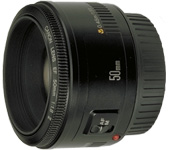
\includegraphics[width=0.49\textwidth]{canonef50mm-1}%
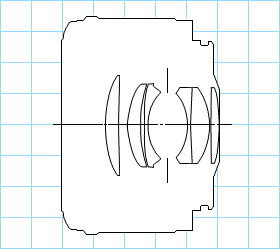
\includegraphics[width=0.49\textwidth]{canonef50mm-2}
}{fig:canonef50mm}{
	A fixed focal length Canon EF 50mm f/1.8 II camera objective.
	Left: the device, not attached to a camera.
	Right: block diagram of the lens construction, showing the six optical elements.
	Diagram by Canon Camera Museum \cite{canonmuseum50mm}.
}


\simplefig{t}{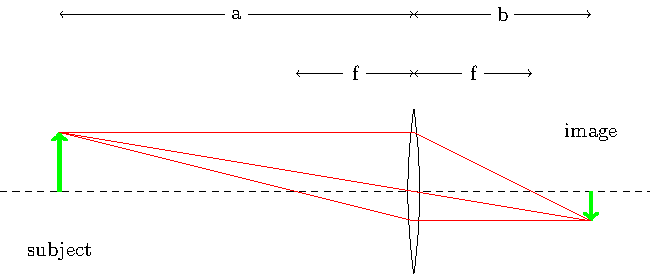
\includegraphics{lens}}{fig:thinlens}{
	thin lens sample: $a=6$, $b=3$, $f=2$.
	Actual subjects would be usually much further away; image depicts a macro setup for clarity.
	A subject at a distance $a$ is \emph{focused} on a film at a distance $b$ on the other side, as light rays (red) travel via the lens.
}

\paragraph{Focusing}
A point on a subject is said to be \emph{in focus} when the light rays originating from it converge at the same point on the camera's film.
When the camera objective is adjusted for the object to be in focus, its parameters are changed slightly and a different thin lens is formed.
\emph{Focal length} is a fundamental property of a lens and determines its amount of magnification \cite[p.~61]{szeliski10vision} \cite[p.~13]{greenleaf1950photographic}.
Illustrated in Figure \ref{fig:thinlens}, the thin lens model and its focal length $f$ encode a relation between an object at a distance $a$ and its \emph{focused} image at a distance $b$ on the other side, as shown in Equation \ref{eq:thinlens}.
A camera system typically has a \emph{magnification} of much less than one, i.e., the image on its film is rendered smaller than the imaged subject, as $a \gg b$.
For objects at distances approaching infinity ($a = \infty$), $b$ becomes equal to $f$, and the thin lens resembles a pinhole with film distance $f$.
\begin{equation} \label{eq:thinlens}
	\frac{1}{a} + \frac{1}{b} = \frac{1}{f}
\end{equation}

% Aperture, its effects (light, dof...)

\paragraph{Aperture}
The size of the hole where light effectively goes through is called \emph{aperture}; the hole itself is called \emph{aperture stop} and it is located inside the the objective in between its lenses.
The diameter of a thin lens corresponds to the aperture diameter and to the stop's \emph{entrance pupil}, the aperture stop seen from the front of the objective.
Size of the aperture also directly determines the amount of light entering the image plane, and thus the relative exposure time for a required amount of light energy: doubling the aperture area halves the required exposure time.
\cite[ch.~13]{greenleaf1950photographic}

% TODO: dof graph: varying distance, N lines for different f/#
As in any practical case, the aperture is not infinitesimally small, and there will be some area of the scene that is imaged as sharp and others in front and behind of this area will be blurred.
This effect is called \emph{depth of field (DOF)} and is illustrated in Figure \ref{fig:irldof}.
In artistic photos, a \emph{shallow} depth of field can be preferred, having the subject in focus to separate it from the background by blurring.
In 3D reconstruction, exactly the opposite is preferred: deep focus, i.e., objects at every depth from the camera should be sharp.
The aperture size is presented as relative to the focal length and is commonly called the \emph{F number, $N$} \cite[p.~23]{greenleaf1950photographic}, specified via the aperture diameter $d$:
\begin{equation} \label{eq:fnumber}
	N = \frac{f}{d}
\end{equation}

\simplefig{t}{%
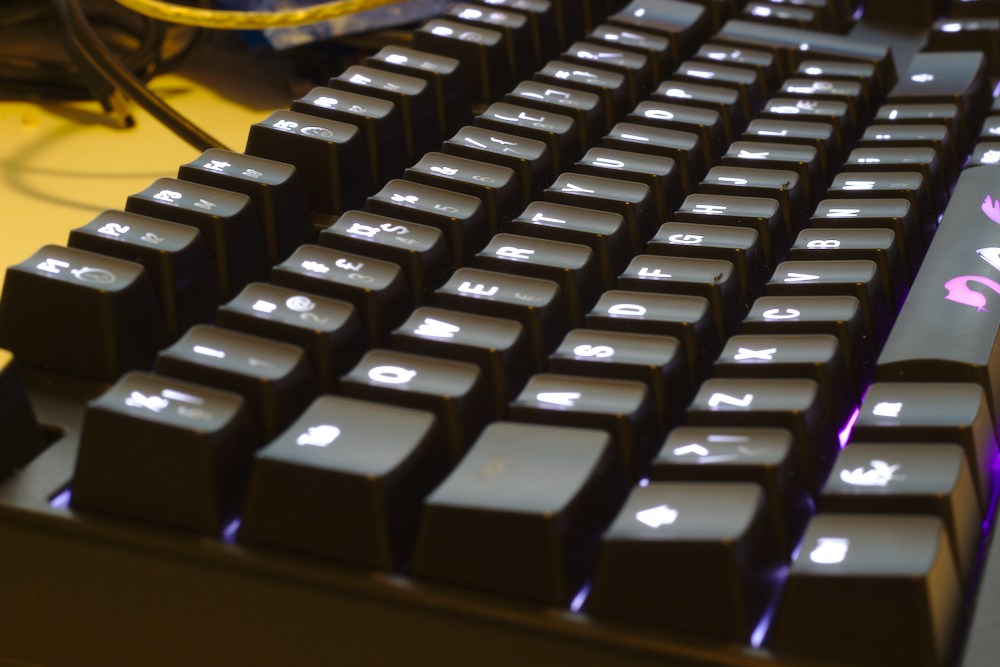
\includegraphics[width=0.45\textwidth]{irldofdeep}

\includegraphics[width=0.45\textwidth]{irldofshallow}
}{fig:irldof}{
	Deep and shallow depth of field in close-up photography using a 50 mm lens.
	Left: f/16 aperture, 15 second exposure, showing only slight blur in the nearest keys.
	Right: f/1.8, 0.2 s exposure, with only a small sharp area.
	The image blurs and the distinctively brighter small lamps on the keys show as increasingly larger bright spots as the circle of confusion increases.
}
Clearly, doubling the area of the aperture equals to an increase of the diameter $d$ by a factor of $\sqrt 2 \approx 1.4$.
The aperture size is typically denoted literally as $f/N$, such as $f/1$ or $f/1.4$.
This makes the light energy reaching the film universal among all focal lengths.
Full multiples of $\sqrt 2$ are called \emph{stops}, and the perceived f number changes as a function of subject distance \cite[p.~23]{greenleaf1950photographic}, which is left out here for simplicity.

\paragraph{Circle of confusion}
As the blur happens gradually, the ``level of sharpness'' at each point is often defined via a \emph{circle of confusion} (CoC) \cite[p.~25]{greenleaf1950photographic}.
The distance from the lens along the optical axis where perfect focus is attained is called the \emph{focal plane}.
Every point nearer or further away shows up on the film as a circle (for circular apertures), instead of a point; when this circle is significantly larger than the resolving power of the observer, the image of this point is perceived as blurred as the image is the integral of all of these circles.

Depth of field is defined as difference between the shortest and farthest object distances that still generate an acceptable CoC, found geometrically.
When $f$ is the focal length, $N$ the aperture f number, $s$ the distance to the subject, and $c$ the maximum acceptable CoC, the depth of field $D$ is (Greenleaf \cite[p.~25]{greenleaf1950photographic}):
\begin{equation} \label{eq:dof}
	D = \frac{2 s f^2 N c (s - f)} {f^4 - N^2 c^2 (s - f)^2}
\end{equation}

\simplegfx{t}{\textwidth}{dofcoc}{
	Depth of field and circle of confusion with a thin lens, seen from the side (not drawn to scale).
	Subjects at distance $s$ project perfectly at the film.
	Distances between $Z$ and $Z'$ project to a circle smaller or equal to $c$.
	It is easily seen that for subjects at longer distances, the depth of field increases.
}

In Figure \ref{fig:dofcoc} that depicts the formation of the circle of confusion, $Z'$ and $Z$ are the maximum and minimum acceptable distances near the subject, and $Z' - Z = D$.
Sufficient depth of field is important in near-field 3D scans, which translates to a small aperture, and consequently, relatively bright lights in order to maintain a short exposure time.
The subject should fill whole image frame to use the pixel density effectively.
Increasing the distance to the subject would increase depth of field, but enlarging the subject in the frame again would need a higher focal length, which decreases depth of field.

Acceptable size of the CoC depends on the resolving power of the viewer; when a photograph is looked at, the print size and distance of the viewer determines the circle \cite[p.~26]{greenleaf1950photographic}.
A standard-considered formula in photography determines the maximum acceptable CoC by dividing the image size by 1500, originating from human vision performance \cite[p.~88,~92]{kingslake1992optics}.
As an example, for the standard ``full-frame'' 35 mm film size with an image size of 36 x 24 mm (approx.\ 43 mm diagonal), the CoC yields $c = 43 \text{ mm} / 1500 \approx 0.03 \text{ mm}$.
For a normal 50 mm lens with the subject at a distance of 1 m, a small aperture of f/11 and using a circle of confusion of 0.03 mm, Equation \ref{eq:dof} gives depth of field of $D \approx 25 \text{cm}$.

In a computer vision system, this purely perceptual guideline is typically ignored and the circle of confusion is determined by the sensor resolution or pixel size.
The disk should not span too many pixels, so that accurate detail would be resolvable from the digital image.
The pixel size is typically in the order of micrometers, with which a much smaller CoC is required.
The sensor of Canon EOS 1D X, for example, has a pixel size of approximately $7 \times 7$ micrometers \cite{eos1dx} which is considered large.
When properties such as type of the subject texture and the quality of the optical path to the sensor influence the resolving power, the circle of confusion is typically used as a guideline instead of a strict rule.

% diffraction

\paragraph{Diffraction}
The required amount of light is not the only factor that limits the minimum aperture size.
\emph{Diffraction} is an effect which reduces image sharpness with small apertures.
When a light ray diverges on a small aperture due to the wavelike nature of light, the different distances traveled make the rays interfere each other and produce a two-dimensional diffraction pattern, called an \emph{airy disk} \cite[ch.~4]{greenleaf1950photographic}.
The disk blurs the image in a similar fashion as an object that is out of focus, as each light ray produces its own particular disk.
Size of the airy disk is relative to the size of the aperture and the light wavelength.
Thus, the aperture size must be chosen as a compromise between the unwanted effects of DOF and diffraction.
The disk size can be approximated \cite[p.~29]{greenleaf1950photographic} by
\begin{equation} \label{eq:airydisk}
	c = 1.22 \frac{\lambda f}{d} = 1.22 \lambda N
\end{equation}
which, for example, for red light having a wavelength $\lambda$ of 700 nanometers, with an aperture of f/11, results in $\approx$ 0.01 mm (compare to above CoC of 0.03 mm).
Again, this should be compared to the image sensor's pixel size, and already an aperture of f/11 would approach the diffraction limit.

\paragraph{Geometric distortion}
While most rectilinear lenses are close to a perspective projection, practical optical systems introduce some non-linear \emph{radial} and \emph{tangential distortion} that affect the accuracy of the ideal pinhole model as light rays travel through the pieces of glass \cite{brown1966decentering,brown1971close}.
Common distortions are the purely radial so-called \emph{barrel} and \emph{pincushion} distortions, where the lens magnification is a nonlinear function of image ray distance from the center of the lens, caused by the shape of the lenses \cite{brown1966decentering,brown1971close}.
In addition to radial, tangential distortion is less significant, and it is often ignored.
Its cause is small misalignments in separate elements in a single optical system, lenses being offset from each other and not being parallel to the image plane \cite{brown1966decentering,kingslake1989history}.

\simplefig{t}{%
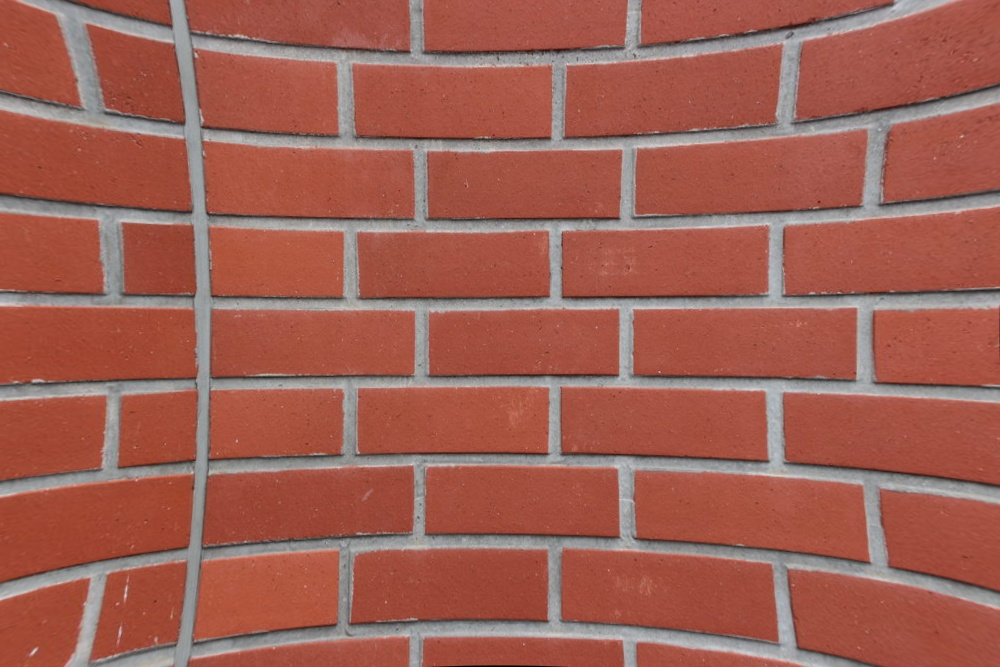
\includegraphics[width=0.32\textwidth]{wall-pincushion}
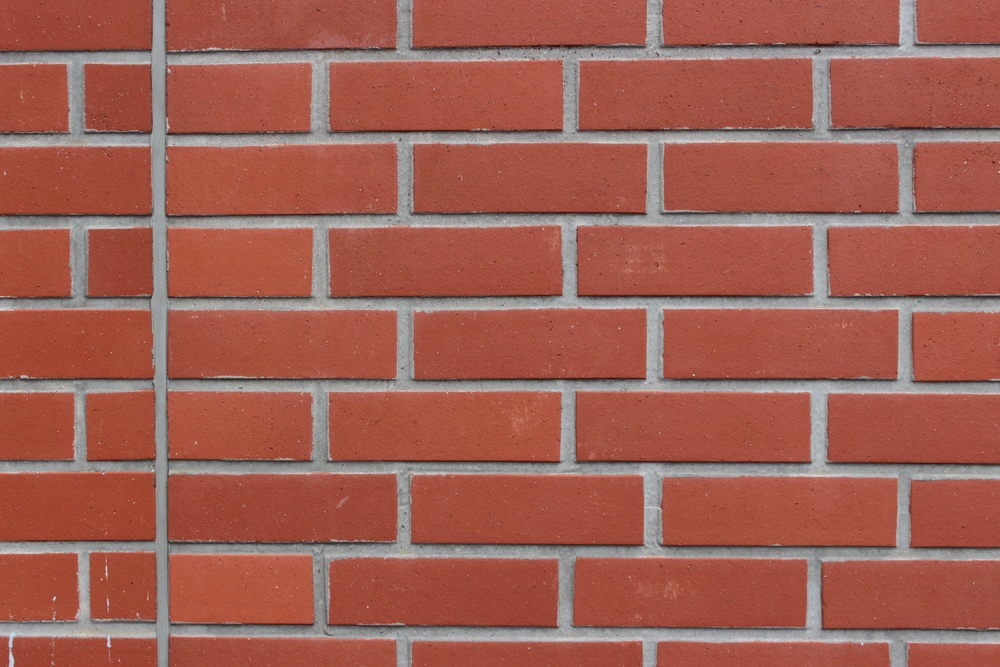
\includegraphics[width=0.32\textwidth]{wall}
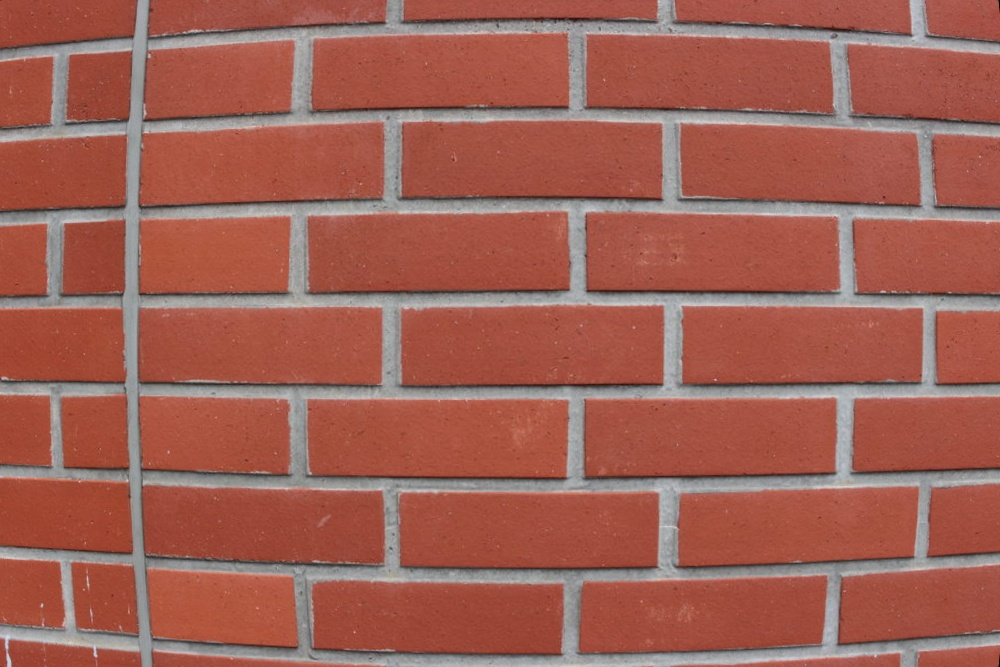
\includegraphics[width=0.32\textwidth]{wall-barrel}
}{fig:distortions}{
	Simulated pincushion (left) and barrel (right) distortions by applying undistortion on an undistorted image (center) using OpenCV.
}

Because stereo vision assumes that the images are free of nonlinearities, i.e., straight lines in the world should remain straight in 2D images after the projective transformation, it is important to correct the geometric distortions beforehand \cite{szeliski10vision}.
The radially symmetric radial error model and correction proposed first by Brown \cite{brown1971close,brown1966decentering} and used directly or with slight alternations in programming libraries, e.g., OpenCV \cite{opencv}, is
\begin{align} \label{eq:radialdist} \begin{split}
	x_{corr} &= x(1 + \kappa_1 r^2 + \kappa_2 r^4 + \kappa_3 r^6)\\
	y_{corr} &= y(1 + \rho_1 r^2 + \kappa_2 r^4 + \kappa_3 r^6).
\end{split} \end{align}
where $x$ and $y$ are the original coordinates in the distorted image on the film or image sensor, $x_{corr}$ and $y_{corr}$ are the corrected ones, $\kappa_1$, $\kappa_2$, $\kappa_3$ are coefficients specific to the radial distortion and $r$ equals to the distance to optical origin, located at $(x_c,~y_c)$:
\begin{equation}
r = \sqrt{(x - x_c)^2 + (y - y_c)^2}
\end{equation}

Trucco and Verri \cite{trucco1998introductory} present only the two first coefficients, and it is not rare to use only the first $\kappa_1$; for lenses with low distortion, this is often enough.
A complete derivation of the model involves detailed trigonometric analysis of thin prism models on lens elements \cite{brown1966decentering,brown1971close}, which results simply in Equation \ref{eq:radialdist}, a simple polynomial.
For tangential-only distortion, the corresponding correction has the following form:
\begin{align} \label{eq:tangdist} \begin{split}
x_{corr} &= x + 2 \rho_1 x y + \rho_2 (r^2 + 2 x^2)\\
y_{corr} &= y + 2 \rho_2 x y + \rho_1 (r^2 + 2 y^2)
\end{split} \end{align}
where $x$, $y$, $x_{corr}$, $y_{corr}$ and $r$ are as in Equation \ref{eq:radialdist} and $\rho_1$ and $\rho_2$ are new coefficients specific to tangential distortion.

The two independent types of distortion are combined by summing them both to the original coordinate, combining Equations \ref{eq:radialdist} and \ref{eq:tangdist}:
\begin{align} \label{eq:bothdist} \begin{split}
	x_{corr} &= x (1 + \kappa_1 r^2 + \kappa_2 r^4 + \kappa_3 r^6) + 2 \rho_1 x y + \rho_2 (r^2 + 2 x^2)\\
	y_{corr} &= y (1 + \kappa_1 r^2 + \kappa_2 r^4 + \kappa_3 r^6) + 2 \rho_2 x y + \rho_1 (r^2 + 2 y^2)
\end{split} \end{align}
The effects of different parameters are depicted in Figure \ref{fig:raddist}.
The image dimensions are usually normalized such that the origin lies at the image center, and the distance $r$ from the center has a maximum value of $1$, making the distortion parameters universal for all image resolutions.
A typical image sensor is not a square but a rectangle, and clips the distortion circle accordingly, such that the maximum coordinates along the different axes are different.

\simplegfx{t}{\textwidth}{raddist}{
		Purely radial distortion correction with different values of two parameters.
	The arrows point from original coordinates $(x, y)$ to corrected ones $(x_{corr}, y_{corr})$.
	From left to right: $\kappa_1 = 0.16$, $\kappa_1 = -0.16$, $\kappa_2 = -0.08$, $\kappa_1 = -0.04, \kappa_2 = -0.04$.
	The different shapes of second and fourth order polynomials are easily visible: the higher-order terms are visible have most effect in the farthest sides of the image.
	The leftmost correction is for a barrel distortion, and the others are for pincushion distortion.
}

The Brown's model describes the distortion characteristics for a lens system on an otherwise perfect image, but typically the inverse transform is required, because a distorted image is given as noted by e.g.\ Villiers et~al.~\cite{villiers2008centi}.
For each pixel in the undistorted destination image, the pixel value is necessary to find from the distorted source, but the mapping described by the model works to the other way.
However, Villiers et~al.\ note that as plain barrel and pincushion distortion can be considered as inverse transforms to each other, the same model can actually be used for the inverse direction if the more complex tangential part is left out \cite{villiers2008centi}.

Because digital images consist of a discrete pixel array, the pixel coordinates given by the undistortion do not necessarily lie on exact pixel positions; the sampling should then interpolate between neighboring pixels, considering the image as a continuous but discretely sampled 2D function \cite{wolberg1990digital}.
Throughout this thesis, interpolation is assumed to be performed as necessary when sampling an image.

%Normal TV is usually watched at the distance of twice the screen diagonal.
%At this location, the scene looks normal when taken with a normal lens.
%A wide-angle scene then looks normal when viewed at a nearer distance. \cite{wilson2004anton}
% 14:01:55 <naavis> Kai sillä yritetään emuloida sitä, että katsojan paikalta se leffan kuvakenttä vastais sitä että valkokankaan tilalla on ikkuna.

% }}} optics

\subsubsection{Shutter} % {{{

% shutter, why needed

A static scene is imaged by exposing the photosensitive film (or digital sensor) to the light passing through the optics for a short time, keeping the camera and subject steady.
A \emph{mechanical shutter} blocks the light before and after the exposure \cite[ch.~13]{greenleaf1950photographic}.
In recent digital image sensors, the sensor itself can be made inactive to light or cleared quickly from the accumulated charge; this is called \emph{electronic shutter} \cite{caspeelectronic,kodakshutter}.

% mechanical stuff

\simplegfx{p}{0.99\textwidth}{focalplaneshutter}{
	Focal plane shutter has two moving curtains to cover the film, opening it momentarily so that each part of the film receives light for the same amount of time.
	From left to right: initially, the film (grey) is blocked.
	Once the first curtain (shown in red) moves away, the film is exposed to light.
	A second curtain (shown in blue) stops the light from entering again.
	The shutter resets by moving back to the initial position.
}

\simplegfx{p}{0.99\textwidth}{focalplanerolling}{
	Rolling shutter effect in a focal plane shutter happens when the exposure time is short relative to the curtain speed.
	The curtains have to move at the same time, exposing only a part of the film at a time.
	Fast subject movement during the exposure leads to artifacts and a rapid flash light would illuminate only a part of the film.
}


\paragraph{Shutter types}
All shutters serve the same purpose: to restrict light from entering the image plane before and after the exposure.
There are several types of constructions for shutters, depending on the application.
Some cheaper compact cameras have a small \emph{diaphragm shutter}, or \emph{leaf shutter} in the lens center near the aperture stop.
A leaf shutter moves quickly away from the light path and back, either as a single opaque piece or as several \emph{leaves}, analogously to the aperture stop whose size can be changed \cite[p.~117]{greenleaf1950photographic}.

A \emph{focal plane shutter} \cite[p.~123]{greenleaf1950photographic}, used in most system cameras, is installed in front of the film plane.
Leaf shutters would be expensive to install in each interchangeable lens, and a focal plane shutter can operate at higher speeds.
Focal plane shutter consists of two curtains that move to the same direction; one moves out of the way of the film to let light pass to it, and another moves to cover it back again when the exposure time has elapsed.
Figure \ref{fig:focalplaneshutter} illustrates the working principle of a planar shutter.
In film cameras, the focal plane shutter was originally two fabric ``curtains'';
today, they are constructed from small, interleaved metal or plastic sheets.

Some cameras have only an \emph{electronic shutter} instead of moving parts.
Electronic image sensors can only be cleared and read out at a restricted rate, and their operation is similar to a focal plane shutter.
\cite{caspeelectronic,kodakshutter}

Video film cameras that capture each frame to a separate part of film used a spinning wheel with a transparent window, called rotary disc shutter \cite{wilson2004anton}.
This rotates at a precise speed synchronized to the frame rate, exposing the film to light for a consistent duration for each frame.
The size of the window constitutes to the amount of light and motion blur.
Video is more discussed in Section \ref{sec:video}.

\paragraph{Artifacts}
If the camera or the imaged subject moves while exposing the frame, the subject gets smeared along the movement on the image, an effect known as \emph{motion blur}.
A related \emph{rolling shutter} effect is produced using a focal plane shutter with very high speeds, where the limit of curtain speed prohibits fully opened shutter.
The closing curtain starts to move before the first has stopped, exposing only a narrow band of the film at a time.
Fast mechanical shutter movement is depicted in Figure \ref{fig:focalplanerolling}.
When an object is moving to the same direction as the narrow shutter slit, i.e., vertically, it appears smeared;
when the movement is horizontal, the subject appears to bend.
An electronic flash light that outputs a very brief pulse of high-intensity light also cannot be used with high focal plane shutter speeds, as it would illuminate only a narrow slit of the sensor.
Electronic shutters also suffer from a similar effect; this is more discussed in Section \ref{sec:sensors}.
Since a leaf shutter opens radially near the aperture stop, it does not have this effect, and it can be used at higher speeds with flash lights.
Leaf shutters suffer from another artifact:
at higher speeds, the longer time spent covering the far sides of the image leads to uneven brightness.
Result of shooting a moving object with rolling shutter is depicted in Figure \ref{fig:rollingeffect}.
A ruler was attached to a rectangular plate, and moved left by hand aligned to a table, with different shutter speed and sensitivity settings.
Skew induced by rolling shutter is visible always, whereas motion blur is reduced with a faster shutter speed.

\simplefig{t}{%
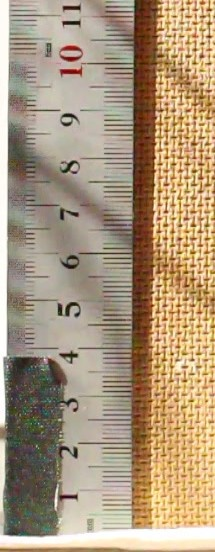
\includegraphics[width=0.3\textwidth]{rollstationary}

\includegraphics[width=0.3\textwidth]{roll100}
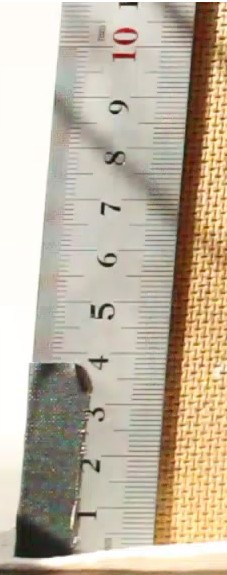
\includegraphics[width=0.3\textwidth]{roll4000}
}{fig:rollingeffect}{
	Motion blur and rolling shutter in a ruler, moving left.
	The ruler does not actually skew or tilt physically; it is vertical and rectangular at all times, but appears skewed.
	Left: a stationary ruler.
	Middle: 1/100 s shutter speed. % , ISO 100.
	Right: 1/4000 s shutter speed. %, ISO 6400.
	Camera aperture was set to f/8; the pictures are cropped from 720p video recorded with a Canon EOS 700D.
	(Color filter and low sampling rate artifacts are visible as color errors in the high-contrast lines of the ruler.)
}

% FIXME z left handed?

% other

\paragraph{Lag}
When taking a picture by pressing a button, the camera does not instantly start to expose the image.
Each camera has a specific \emph{shutter lag} that is the time that elapses between when the shutter button is pressed and when the actual exposure starts to happen.
Some sources include in this term also the time for the camera to perform autofocus and measure sensitivity settings which can take a significantly longer and unpredictable time.
Shutter speed has also small variations over time when the camera ages and mechanical parts wear out.

Some difference also exists among same camera model from mechanical variations and software processing.
Shutter lag of consumer devices typically varies between tens to hundreds of milliseconds \cite{hasshutterlag}.
% }}} shutter

\subsubsection{Image sensors} \label{sec:sensors} % {{{

% intro: film vs sensor, what is a camera

Historically, photographs were saved on a photosensitive film.
With digital cameras, a rectangular electrical \emph{sensor} replaces the film.
The sensor consists of a uniformly spaced grid of small sites that convert the visible optical image to electrical signals, built as an integrated circuit package.
In conjunction with the digital signal processing in the camera, the sensor produces a digital image file.

% pixels, colors

As introduced in the beginning of this section, digital images are represented as arrays of colored pixels.
In order to obtain an appropriate image, the sensor must capture the light it sees also as a discrete array.
The separate red, green and blue color bands are captured in color cameras with separate parts of the sensor, as will be explained.

\paragraph{Photosites}
A sensor consists of individual photosensitive semiconductor sites that each accumulate charge and ultimately encode a single numerical value, relative to the amount of light received \cite[ch.~3]{nakamura2005image}.
Physical pixels cover less than the full area of a sensor, as there are gaps between them;
microlenses between the sites direct the light hitting the gaps to the neighboring pixels in modern sensors, with varying color performance \cite[p.~64]{nakamura2005image} \cite{el2005cmos}.
%Because of the discrete nature of the pixel array, some cameras use an analog low-pass filter in front of the sensor to hide high-frequency information that would show up as aliasing.

A single pixel sensor acquires all light hitting it, independent of the wavelength.
The most common method to capture the three primary colors is to interleave red, green and blue colors in a single sensor by filtering the wavelength that can enter each pixel with a colored film over the sensor, with a special repeating pattern called \emph{color filter array}.
The missing values for other colors bands are interpolated from surrounding pixels.
The most popular interleaving pattern is the Bayer filter \cite[p.~76]{szeliski10vision}, illustrated in Figure \ref{fig:bayerpattern}.
Other arrangements than red, green and blue are also used; e.g., red, green, blue and emerald or cyan, yellow, green, and magenta \cite{park2003implementing}.
Alternatives have slightly better color accuracy at the expense of spatial resolution.

\simplefig{t}{\bayer{0.6}}{fig:bayerpattern}{
	A small partly drawn subset of the repeating $2 x 2$ Bayer pattern.
	Each square represents a single pixel; the colored pattern on top filters the light per each pixel on the sensor array.
}


\paragraph{Sensor technologies}
Near the raw pixel sensors is analog and digital logic for converting and reading out the data and passing it to an image processor.
Quality and type of this conversion affects some properties, most important of which are analog-digital converter noise and dynamic range, and speed at which the image is read out from the sensor.

Two major sensor types exist: CCD (Charge-coupled Device) and CMOS (Complementary Metal-Oxide Semiconductor).
The types vary by their manufacturing techniques and photosite internals \cite{nakamura2005image,taylor1998ccd,el2005cmos}.

Both CCD and CMOS have their applications, but it suffices to say that CMOS is the one used in most still cameras because of its lower price and power consumption, and higher speed.
A CMOS sensor converts light immediately to voltage, and has additional transfer circuitry at each pixel, reducing the \emph{fill factor}, the sensitive parts of the photosites \cite[p.~62]{nakamura2005image}.
In a CCD, the charge is first stored as electrons as in a capacitor, and a row is transferred serially from pixel to pixel to a separate voltage converter and amplifier.
Still, both are typically read out ultimately in a serial fashion, requiring longer reading time for larger amounts of pixels.
A CCD typically uses additional photosites permanently blocked from the light for storing the accumulated charge temporarily.
A CMOS sensor, on the other hand, cannot easily employ additional storage pixels, and is read sequentially, making the reading process resemble the rolling shutter effect.
Rolling shutter is especially noticeable in videos shot with a CMOS camera, because a mechanical shutter is not used for video and the readout process is relatively slow \cite{taylor1998ccd,caspeelectronic}.

\paragraph{Error sources}
Various steps of the image processing contribute to image noise; the major sources are shot noise and several electrical noises \cite{szeliski10vision,litwiller2001ccd}.
\emph{Shot noise} exists due to the particle-nature of light; each photon adds a constant electrical charge to the photosite it hits, and if the overall number of photons is small, statistical Poisson-distributed noise will be present \cite[p.~74]{nakamura2005image}.
This type of noise is visible in less bright areas.
Clearly, no electronically better sensor can improve the visibility of shot noise.
The only way to reduce it is by exposing the sensor to more light: for this reason, sensors with a larger surface area are preferred in applications where noise is unwanted.

The Gaussian-distributed \emph{electrical noise} has various sources in sampling, transfer and conversion.
Each pixel receives an additional random signal level that shows up as additive brightness, also noticed usually only in poorly illuminated conditions or dark areas.
Noise increases with sensor's signal gain, or \emph{exposure sensitivity}, described using the ISO system (``film speed'').
Sensor \emph{responsivity} usually refers to the raw signal the photosite sensor produces per unit of optical energy \cite[p.~78]{nakamura2005image}.
The resulting digital value depends on this and many other terms on the signal path.

A more sensitive ISO setting on a sensor requires less light for a bright-looking image, because the signal is amplified more before digitization.
This amplification also amplifies the original signal noise.
Additionally, the reduced exposure time allows the shot noise to be more visible.
Due to these reasons, the gain level should be kept as small as possible and the amount of light entering the sensor as large as possible.
This leads to requiring bright lighting in the imaged scene or a longer exposure time.
Higher ISO should be used only if shorter exposures are desired due to a moving subject.
Better sensors advertised as more responsive to light typically have larger sensors or less noise-sensitive circuitry, resulting in higher signal to noise ratio \cite{el2005cmos}.

Photosites may also accumulate leaking charge on their own even though no light is entering the site because of \emph{dark current} \cite{el2005cmos,litwiller2001ccd}.
Additionally, the analog-digital converter introduces \emph{quantization error} where an analog signal is not perfectly represented by a discrete number; with the high bit depth of modern sensors, this is practically not an issue.
A high bit depth also presents larger \emph{dynamic range}, i.e., the difference between the brightest and darkest possible representations \cite{el2005cmos,litwiller2001ccd}.

% }}} image sensors

\subsubsection{Lighting} \label{sec:bg-lighting} % {{{

In addition to multiple cameras at different locations and poses to encode a subject's geometry, uniform and soft lighting is also required for consistent color reproduction.
A large variety of different studio lights are available in the market for different lighting situations, emitting either continuous light or bright flashes.

\simplegfx{t}{0.7\textwidth}{nayarbrdf}{
	Polar plots of three reflection components as functions of the viewing angle, as suggested by Nayar \cite{nayar1991surface}, showing the brightness seen from different angles from the surface normal.
	In a reconstruction subject, the bright specular spike and lobe reflections should be minimized, and only the diffuse color is desired.
}

\paragraph{Surface color}
The \emph{perceived} color of a point on a surface is the light exiting it and reaching the viewer.
Therefore, the light sources should be uniformly white and cast no shadows.
Surfaces reflecting light can be modeled as a combination of \emph{diffuse} and \emph{specular} components that are functions of light direction, viewing direction and sometimes additionally location on the surface.
Surface reflection models are described with a \emph{bidirectional reflectance distribution function, or BRDF} \cite{nicodemus1965directional}.
Such distribution model of the surface's global or local microgeometry specifies how much light reflects in different directions \cite{nayar1991surface}.
\emph{Diffuse} means a material that reflects light uniformly to all directions, depending only on the angle between the surface normal and light location, whereas more \emph{specular} surfaces are composed of a different microstructure that reflects light in a mirror-like way; the surface brightness depends on where it is looked from.
In Figure \ref{fig:nayarbrdf}, different types of reflections seen by the camera are visualized as a function of the camera viewpoint.

% XXX pic of brightness constancy: same object from two views, patch windows

\paragraph{Color capture}
Ideally, the camera would only record the diffuse reflection that represents the surface color (\emph{albedo});
any shadows and the specular components are unwanted artifacts from the standpoint of simple color reconstruction.
\emph{Specular highlight} or \emph{specular reflection} refer to a mirror reflection of the lamp on the imaged surface.
Because most reconstruction methods fundamentally assume uniform lighting conditions, a property called \emph{brightness constancy} (i.e., the brightness and color of a surface looks the same, regardless of viewing direction or time moment), they perform poorly when a light shines off a surface differently in different views \cite[ch.~8.3]{trucco1998introductory}.
As images describe the color via the brightness that reflects off of a surface, the perceived brightness must be held constant.
The same restriction provides a basis to other algorithms, such as object tracking \cite{horn1974determining,horn1981determining}.
Examples of complex surfaces containing much specularity are glossy textures and sweaty human skin.

On the contrary, in photographs and image synthesis, shadows and reflections are natural, and images without them would look odd to the eye; capturing only albedo of surfaces -- the color reflectivity of a surface -- is particular to texture capture in reconstruction.
In practice, polarizing filters may be used in front of the lights and in the camera lenses, to filter out most of the specular lighting.
Advanced capture and rendering methods may take advantage of also the specular component \cite{ghosh2011multiview}; however, capturing material properties is easily done separately from the geometry capture \cite{aittala2013practical}.

\paragraph{Light sources}
As the surface should be illuminated as evenly as possible to minimize specular highlights and shadows, it is important to pay attention to light sources.
The often used photography terms \emph{soft} and \emph{hard lighting} refer to the size and power of light sources: bright spotlights are hard, and larger and relatively less bright lamps are soft.
Softness can be added by increasing the light's area while holding its power constant using a ``diffuser'', such as a large surface where light is reflected off or a white cloth between the lamp and the imaged subject.
\cite[p.~108]{langford2000basic}
% TODO Effects of a soft versus hard light are illustrated in Figure \ref{fig:lighthardness}.

Powerful electronic flash units use usually a gas-filled tube that is excited with high voltage to produce a short, bright burst of light for some milliseconds;
since this tube is small, a diffuser should be used for uniform lighting.
Flashes are especially suitable for human subjects, because the subject sees the bright light only for a brief moment; thus, the light does not annoy the subject as continously bright lamps would.
Short bursts of light in an otherwise dark environment are also suitable for stopping motion and synchronizing multiple cameras, as only a short time is effectively exposed to light \cite{langford2000basic}.

% }}} light sources

\subsubsection{Data capture path} % {{{

The image information travels from the subject through the optics to the image sensor's surface, via an analog/digital converter, the camera's processor(s) and finally to mass storage \cite{szeliski10vision}.
The final mass storage is typically on the camera in consumer devices, or on a computer reached by a wired connection for more sophisticated machine vision cameras \cite{hornberg2007handbook,ni2013choosing}.
Many parts in this path contribute to the quality of images and the rate at which the images can be taken, usually measured in frames per second (FPS).

% fps, performance sample

For example, for the high-end Canon DSLR camera EOS-1D X, a continuous shooting speed of 14 frames per second is advertised \cite{eos1dx}.
With its resolution of 5184 by 3456 pixels and 14-bit processing, an estimate for the bit rate from the sensor is
\begin{equation} \label{eq:eos1dspeed}
5184 \times 3456 \times 14 \times 14 \approx 3.5\text{ Gb/s}
\end{equation}
by average, or 0.4 gigabytes per second, requiring also high speed from the processor and mass storage.
Due to the cost of transferring and processing large amount of data, video is typically recorded in lower resolution for faster FPS.

% files

A ``raw'' image file can be saved with more advanced cameras, containing the plain sensor data with very little processing done.
The raw files saved by DSLR cameras are packed in a proprietary lossless format and contain also metadata about certain camera settings.
When a raw file is not used, the camera processes the image with device-specific correction filters and applies image enhancements, e.g., white balance correction and sharpening, and finally saves the image as a standard image file such as JPEG \cite[p.~412]{szeliski10vision}.
For such automatic in-camera processing, all cameras should be identical for consistent reconstruction results.

%Lossless compression maintains image quality and reduces file size depending on the complexity of the frame.
%Some manufacturers encode the brightness values through a lookup table, and it's common to use a compression scheme known from standard file compressions, or a specific lossless image compression.

Video files are almost always saved in a lossy video format by consumer devices, the H.264 format being common for modern cameras.
Compression introduces loss of detail and artifacts typical to the particular algorithm, often visible as blocks or blurring \cite{richardson2004h264}.
Reconstruction quality from frames extracted from such a compressed video may not be as high as from separately saved stills that encode more spatial information.
Machine vision cameras and some professional video cameras can record raw uncompressed video, and some others can be unofficially enhanced;
Canon DSLRs can be tricked using a third-party software modification \cite{magiclantern} to capture the raw stream to a mass storage card, but only some models support the cards necessary for the high recording speed.

% }}} image download

\subsection{Video} \label{sec:video} % {{{

% NOTE ALL-I (intra) / IPB (intra-predict-bidirpredict)

% intro, connection to reconstruction

\emph{Video} is ordered electronic pictures displayed one after another.
Humans perceive \emph{motion} when a previously seen object is seen again in a nearby location.
Current digital video technology encodes motion pictures as in films, in a sequence of still images, recorded and displayed at a constant rate.
Three-dimensional motion is generally no different: it is encoded as discrete poses in sequence.
In order to do motion capture in stereo vision, video material from two or more of cameras is used to initially capture a sequence of still photos.

To reconstruct the frames in 3D, each set of frames encoded by the cameras should be \emph{synchronized}, i.e., shot at the same time, to fulfill the reconstruction assumption of a static subject.

% }}}

\subsubsection{Sequence of frames} % {{{ or: video is frames

% how/when frames are captured
When scanning a scene continuously, a camera shoots frames using the same principles as in photos, but does it in sequence, at a speed that is called \emph{frame rate} \cite{poynton1996technical}.
For each frame, the shutter is open for a duration of \emph{exposure time} or interchangeably \emph{shutter speed}.
In \emph{interlaced video}, two frames make up a whole picture that covers all pixels.
Interlacing alternates between odd and even lines to increase update rate, and was invented for cathode ray tube displays to reduce apparent flicker \cite{poynton1996technical}.
The alternation results in tearing artifacts when imaging horizontally moving subjects (shown in Figure \ref{fig:interlace}).
Many CCD video cameras still produce interlaced stream.
Video that contains full frames only is called \emph{progressive}.

\simplegfx{t}{0.7\textwidth}{interlace}{
	A cropped area of interlaced scanning.
	From left to right: even lines only, odd lines only and full picture combined.
	Top: stationary square.
	Bottom: a moving square, showing tearing if the frames would be combined.
}

% on fps

Consumer video cameras, video-capable pocket cameras and DSLRs typically offer a few choices of frame rate.
Traditionally, the movie industry has used 24 FPS; 25 and 30 are common alternatives used in TV broadcast, some cameras being capable to twice the speed at a lower resolution.
Actual FPS is slowed down from the advertised by a factor of 1.001 because of historical reasons.
30 and 24 FPS refer to approximately 29.970 and 23.976 FPS, respectively.
\cite{musburger2010single}

Externally triggered cameras can clearly be configured to record at any arbitrary rate and exposure, as long as it is in the limits of the camera speed capabilities.
Synchronized machine vision cameras do not record video on their own, but instead monitor a clock signal and output frames at the clock rate.
The frames are then recoded to a computer using \emph{frame grabbers} for interfacing with the cameras.
\cite{hornberg2007handbook}

% dslr sucks

DSLR video modes use almost the sensor's full size but skip some of its lines when recording video, resulting in the same field of view as still images but suffering from significant aliasing patterns with certain subjects with high frequency information.
An alternative would be to crop a smaller part of the sensor for the frames.
Additionally, pixels in the video frames do not represent physical pixels anymore, posing awkwardness in camera calibration.
Line skipping is depicted in Figure \ref{fig:lineskipping2}.
The color filter array makes the problem even worse for small-detailed features of high color detail.

\simplegfx{t}{\textwidth}{lineskipping2}{
	Line skipping in a DSLR camera in video mode.
	Left shows a part of the full sensor and its bayer pattern; on the right, only every third line is captured.
}

% }}}

\subsubsection{Frame rate and shutter speed} % {{{

% no particular reason to be inline instead of pdf, just legacy
\simplefig{t}{
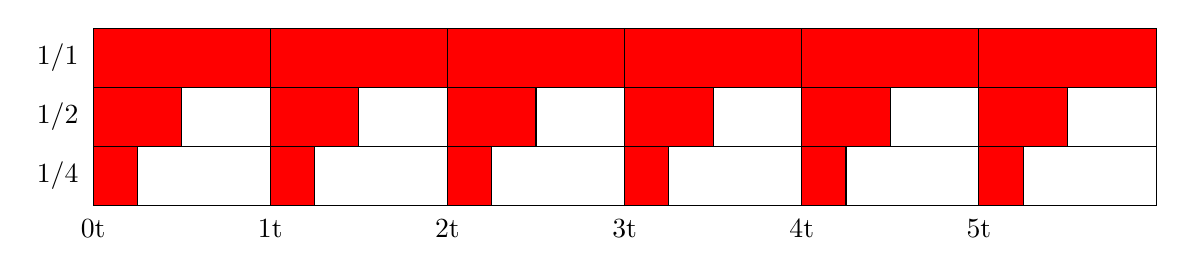
\begin{tikzpicture}[scale=1.5]
	\def\nframes{5}
	\def\w{1.5}
	\draw (0,0) rectangle ++(\nframes*\w+\w,-1.5);
	\draw (0,-0.5) -- ++(\nframes*\w+\w,0);
	\draw (0,-1) -- ++(\nframes*\w+\w,0);
	\foreach \x in {0,...,\nframes} {
		% time ticks
		\node at (\x*1.5, -1.7) {{\x}t};

		% exposure blocks
		\draw [fill=red] (\x*\w, 0) rectangle ++(1.0*\w, -0.5);
		\draw [fill=red] (\x*\w, -0.5) rectangle ++(0.5*\w, -0.5);
		\draw [fill=red] (\x*\w, -1) rectangle ++(0.25*\w, -0.5);
	}
	\node at (-0.3, -0.25) {1/1};
	\node at (-0.3, -0.75) {1/2};
	\node at (-0.3, -1.25) {1/4};
\end{tikzpicture}
}{fig:shutterspeed}{
	Varying shutter speed compared to constant frame rate $1 / t$.
	Red rectangles illustrate exposure time, i.e., open shutter.
	For an always open shutter, the sensor would record continuously.
	A ratio of 1/2 is a ``normal'' rate most used in film.
	1/4 would result in slightly less motion blur and less captured light intensity.
}

A higher frame rate results in more accurate representation of motion as a whole, and a faster shutter speed helps to reduce motion blur in individual frames.
For reconstruction, ideal exposure time would be infinitesimally short; practically, the amount of available light restricts the time, even though a camera would be faster.
Similarly, what happens when the shutter is closed is not recorded; ideal frame rate would be faster than any period of motion in the scene.
For motion tracking based on frame differences, a long enough time should be passed for reliable motion direction detection, though.
%Normally, if playback happens at a different rate from the recording, motion is interpolated between different frames or the last appeared frame is used.

In contrast, in motion picture industry the shutter is kept open deliberately so long that fast motion is blurred, because it is considered aesthetically pleasing to human eye \cite{wilson2004anton};
even though the motion is blurred, it appears less jerky and more temporal information about the scene movement is encoded per frame than when exposing infinitesimally short frames, at the expense of spatial resolution.
A typical shutter speed relates to frame rate such that a frame is exposed half of the time between frames \cite{wilson2004anton}.
%Good cameras allow to change the frame rate and shutter speed independently.

Film cameras and some professional video cameras use a rotary disc shutter that has an opaque 180 degree sector.
Having half the exposure time of frame rate is sometimes called ``180 degree shutter'' due to this historical reason \cite[p.~37]{wilson2004anton}.
While the light is blocked, film is mechanically advanced to the next frame.
Digital video analogously downloads data from the image sensor and clears it during this time.

% }}}

\subsubsection{Multi-camera synchronization} % {{{

%Time offset / drift / jitter / lockstep

Concurrent recording of multiple view video is more complicated than shooting still photos simultaneously.
The cameras should be synchronized together to hold their shutters open at the same time during each frame.
An assumption of stereo vision is that the images encode a static scene, i.e., geometrically same objects, which would not hold otherwise.
Lack of proper synchronization can be compensated to some degree with stroboscopic lighting or morphing between recorded frames if hard syncing is not possible \cite{bradley2009synchronization}.

Within the scope of this thesis, synchronization issues can be divided roughly in three sources of error, assuming N cameras each having its own video file with same frame rate: \emph{offset}, \emph{drift} and \emph{jitter}.
With the same frame rate, the frames can be indexed with numbers starting from 0.
Times when the frames taken relative to a global clock is noted as $t_{Ci}$, where $C$ is a camera identifier and $i$ is the increasing frame index.

\emph{Offset} is the time difference of two streams: for an ideal camera $A$ at each frame $t_{Ai}$ for $i$, and an offset camera $B$ at $t_{Bi}$, a constant error $e$ is added:
\begin{equation} \label{eq:timeoffset}
	t_{Bi} = t_{Ai} + e
\end{equation}

Drift is a property of one a camera that advertises to record at some speed and actually works at some other speed.
Similarly for cameras $A$ and $B$, a constant $d$ is added for each frame index $i$:
\begin{equation} \label{eq:timedrift}
	t_{Bi} = t_{Ai} + d i
\end{equation}

Jitter is the random offset $j(i)$ between frames of an ideal camera A and a camera B:
\begin{equation} \label{eq:timejitter}
	t_{Bi} = t_{Ai} + j(i)
\end{equation}

For an actual video camera, drift and jitter are negligible; offset originates from starting the recording at a different time and from camera's internal processing before the recording actually starts.
If the cameras take pictures only when instructed, such as machine vision cameras, a common clock generator becomes another source of error.
Many consumer cameras support a live preview feed when connected to a computer; the feeds can be useful for previewing but jitter would be too significant.
If the offset between two cameras is not an exact multiple of the frame speed, they effectively cannot have any frames that would display exactly the same scene.

Frame accurate offset sync with clapperboards works by matching the clap sound to visual cues in the video, a method well known in film production.
Cameras that record audio to the same video file do not need visual cues and can be synced together by matching the sound streams.
%This is the method used in making movies when editing a final version with multiple cameras used.
Unsynchronized shooting still leaves an offset of at most half a frame between the camera sequences; this most significant sync issue is illustrated in Figure \ref{fig:syncproblems}.

Professional video cameras can be synced to a single clock generator, so that they all operate on the same frequency (i.e., no drift) and phase (i.e., no offset), called \emph{genlocking} or \emph{generator locking}.
Similar method is used when shooting with machine vision cameras that have external trigger input \cite{poynton1996technical}.
Synchronizable camcorders are expensive, and consumer-grade hardware usually lacks all possibilities for proper sync.

\simplefig{t}{
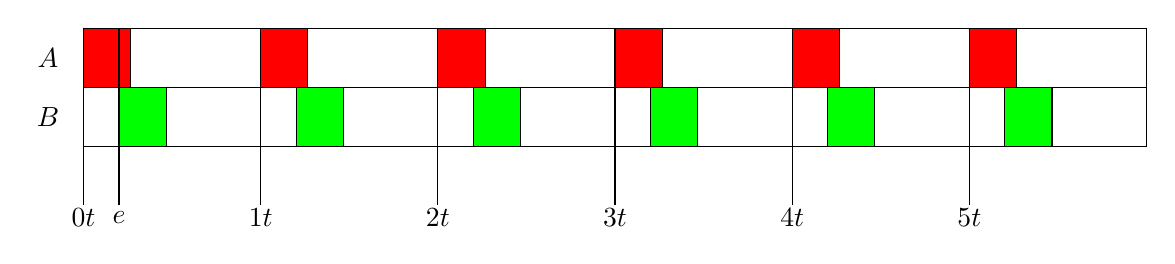
\begin{tikzpicture}[scale=1.5]
	\def\w{1.5}
	\draw (0,0) rectangle ++(5*\w+\w,-0.5);
	\draw (0,-0.5) rectangle ++(5*\w+\w,-0.5);
	\foreach \x in {0,...,5} {
		\draw (\x*\w, 0) -- (\x*\w, -1.5);
		\node at (\x*\w, -1.6) {${\x}t$};

		\draw [fill=red] (\x*\w, 0) rectangle ++(0.4, -0.5);
		\draw [fill=green] (\x*\w+0.3, -0.5) rectangle ++(0.4, -0.5);
	}
	\draw (0.3, 0) -- (0.3, -1.5);
	\node at (0.3, -1.6) {$e$};
	\node at (-0.3, -0.25) {$A$};
	\node at (-0.3, -0.75) {$B$};
	% P, Z
\end{tikzpicture}
}{fig:syncproblems}
{Video phase difference, i.e., offset, illustrated as a timeline.
Red rectangles illustrate exposure times of camera $A$, green rectangles the same for camera $B$.
Frame period is $t$, and the cameras have a constant exposure time offset of an arbitrary $e$.}

% }}}

\subsection{Digital camera types} \label{sec:cameratypes} % {{{

% intro on camera types, wanted options left in implementation

This section quickly reviews the most common types of digital cameras available.
More in-depth survey on properties important in reconstruction are given in Section \ref{sec:cameracomparison}.
%
% camera types introduced

\paragraph{Camera category overview}
\emph{Consumer cameras} have good availability, but they are targeted for artistic photography and basic users.
They are divided roughly in two categories: \emph{compact (pocket, or point-and-shoot) cameras} and \emph{system cameras}.
The presence of a mirror divides system cameras in two: \emph{digital single-lens reflex cameras (DSLR)} and \emph{mirrorless interchangeable-lens cameras (MILC)}.
A MILC lacks a separate viewfinder and the reflex mirror, resulting in smaller size.
System cameras typically support an interchangeable lens and a number of auxiliary hardware, such as electronic flash units, remote shutter releases and power adapters to replace batteries.

\emph{Industrial cameras} for \emph{machine vision}, targeted for engineering applications with high repeatability, are more controllable and contain no unnecessary bulky parts, but are more expensive and inconvenient to set up, and may need proprietary control tools.
Their product cycle is typically longer and thus more reliable than in consumer electronics.
In industrial cameras, the different parts of the system are typically defined more accurately in terms of, e.g., lens quality, sensor and pixel size, sensor noise, processing speed and communication protocol.

\emph{Camcorders}, video cameras with recording capabilities, also vary from consumer to professional grade devices.
Camcorders are not quite considered in this work because of their lower resolution relative to still cameras; many of their benefits lie in user interfaces designed for different purposes in video.
Many still cameras support acceptable video recording.

% some properties

\paragraph{Pixels}
Camera sensor resolution is declared in millions of pixels, or megapixels (MP).
Sensor resolution and image size are related via \emph{pixel size} that is the physical size of one photosite on the sensor.
Pixel size is described as the physical length of one side of a photosite; virtually all sensors today employ square pixels.
System cameras have largest sensors and pixels, and pixel size typically decreases as the sensor size decreases, as manufacturers pursue for high resolution despite of sensor size.
The physical size of the image sensor varies according to use, and ultimately determines resolution, pixel size and light sensitivity.
Currently, typical sensor sizes for different camera categories are as follows:

\begin{itemize}
	\item System cameras use a ``full-frame'' (36 x 24 mm) or APS-C (1.5-1.6x crop of full frame: 22 x 15 mm), resolution usually over 15 MP with pixel size at about 5 micrometres
	\item Compact cameras use a small sensor; sizes vary but are approximately 1/2.3 inch (6.2 x 4.6 mm), resolution about 10 MP or more
	\item Smartphones use sizes between 1/3-1/4 inch (less than 4.8 x 3.6 mm), resolution between 3 to 8 MP
	\item Sizes used by industrial machine vision cameras vary by application, in 5 to 10 mm range having resolutions from 0.5 to over 10 MP.
\end{itemize}

%sensor vibration to remove dust -> sensor position not very fixed \cite{rieke2009}.
%no image stabilizer in sensor or lens \cite{photogrammetry.doc}
%ring flash bending the lens assembly if attached to it \cite{rieke2009}.

% lenses, shutters

\paragraph{Lens quality}
To benefit from the sensor resolution, the camera objective should have an equivalent or better \emph{resolving power}, provided as a chart of \emph{modulation transfer function} (MTF), which is a function of frequency, or number of black-and-white \emph{line pairs} per millimetre.
A lens attenuates the frequencies of the optical patterns, such that at some point, dense line pairs are not resolved from each other but show up as gray.
\cite[p.~71]{kingslake1992optics}

Machine vision cameras and system cameras use interchangeable lenses with often well specified MTFs provided by the manufacturer, while cheaper compact cameras, phones and webcams are designed for a single lens that cannot be removed and has poorer MTF that usually is not provided \cite{sick2006machine}.
Compacts also accompany a \emph{zoom lens} for versatility; zooms are more complex systems and therefore more expensive to reach an image quality comparable to others.
Calibration is also an issue with moving zoom elements that may not align to precisely the same setting.
Interchangeable lenses have a large selection of fixed focal length (``prime'') lenses with less moving parts and typically better optical quality.
The lack of zoom of a prime lens is acceptable in a controlled environment, where the distance to the subject can be adjusted as necessary.
With DSLRs that have a moving mirror and a shutter, the mechanical vibration could move the zoom lens each time a little, changing the focal length.
%Rieke-Zapp et~al.\ \cite{rieke2009evaluation} address several problems in camera calibration and imaging quality.

% storage

\paragraph{Data storage}
Storage size and speed and camera processing power in general follows camera price.
High-quality motion capture of short performances is aided by continuous burst mode that can achieve anything between 2 and over 10 frames per second, depending on camera model.
Professional-level DSLRs and many MILCs can handle over 10 continuous raw full frames per second, while entry-level DSLRs handle around five;
compact cameras are generally slower.
Machine vision cameras with resolutions comparable to DSLRs also exist, but at a significantly higher price.
Overall storage speed is determined by several factors between the sensor, the camera's processor and mass storage.
Reading the pictures to a computer can be done via USB bus or a memory card reader; the latter method is not practical, since the card must be removed from each camera and placed to a reader manually.
Industrial cameras typically have temporary memory for only one frame that is read out immediately via a bus or transfer the read frame from the sensor directly with no buffering.
For video recording, this needs relatively large amounts of auxiliary hardware to save the raw frame feed.
Additionally, either fast hard disks or large amounts of RAM for live data storage would be required.

% software support

\paragraph{Software support}
For a number of cameras requiring identical parameters and control, setting the parameters and downloading pictures manually is not acceptable.
Major consumer manufacturers provide a software development kit (SDK) for controlling their cameras remotely to some degree, and some support a common standard for file access.
For machine vision cameras, manufacturers provide their own software packages, in addition to sometimes specifying that the camera complies to a standard.
The standards specify data formats and buses, image streaming, and control methods.
Key standards \cite{hornberg2007handbook,ni2013choosing} for industrial cameras are:

\begin{itemize}
	\item Camera Link, partly proprietary serial transfer protocol with special cable and connector types
	\item GigE vision, standard interface for video data over gigabit Ethernet connection; licensed so that writing open source software directly based on the standard is not officially possible
	\item IIDC/DCAM, Instrumentation \& Industrial Digital Camera or 1394-based Digital Camera Specification, data format standard used in IEEE 1394 (Fire-Wire) cameras; an open specification
	\item USB3 Vision, a computer vision standard for the USB 3 bus
\end{itemize}

A standard-compliant industrial camera enables to use readily available software, reducing the need for in-house software and protecting from vendor lock-in.
Some of the largest manufacturers that offer standards-compliant cameras are Point Grey, Basler, Allied Vision, and Imaging Source.

% http://www.edmundoptics.com/imaging/cameras/
% store http://machinevisionstore.com/Catalog/ByCategory?category=1&group=1
% http://www.dpreview.com/products/search/cameras

%Coriander \cite{coriander} is a free user interface for controlling IIDC cameras.

% triggering
\paragraph{Remote trigger}
For a multi-camera setup, reliable remote trigger is important.
It must be possible to signal the shutter release remotely for still pictures and video recording.
Industrial cameras are designed to be remotely controllable, and system cameras have input sockets for remote trigger signals.
Others have limited offer, mainly supporting infrared remote if anything.

% camera comparison

\paragraph{Conclusion}
Summarizing for the general feasibility of the most popular camera types in the market:

\begin{itemize}
	\item System cameras with bigger sensors have high light responsivity, excellent configurability with auxiliary hardware available, such as flash units and remote shutter releases, and decent software support.
	\item Industrial machine vision cameras have both small and medium sensors, support interchangeable lenses and need significant amount of additional signal processing hardware, and custom or expensive software to control.
		Video synchronization is usually not an issue, and parameter control has more freedom at the expense of more work.
	\item Compact cameras, designed for the general public for all-purpose point-and-shooting are cheap, have non-changeable zoom lenses and are in general slower.
		Raw images and external utilities are usually lacking.
		Sensor resolution may be less than in system cameras, and high-resolution compact cameras perform worse in low light because of smaller pixel size.
	\item Others (smartphone cameras, webcams) have poorly documented features, cheaper optics and are not configurable properly in general.
\end{itemize}

% }}} camera selection

\clearpage
\section{Static 3D reconstruction} \label{sec:static3d} % {{{

Multi-view stereo reconstruction is one way to recover the structure of a static three-dimensional scene.
In this thesis, a multi-view setup with ordinary digital photo cameras is assumed;
fundamentally different methods, such as laser rangers or light field imaging, are not considered.

A complete reconstruction pipeline consists of many parts of hardware and software.
This section concentrates on the steps of the software pipeline, which is illustrated in Figure \ref{fig:reconstpipeline}.
The subject is broad and this section aims to only describe the main ideas in a nutshell.
For detailed descriptions and analysis, refer to textbooks, e.g., \cite{hartley03multiview,heyden2005multiple,szeliski10vision}.

Images taken with digital cameras are first scanned for distinct features and matched.
To uniquely detect the 3D position of a point in a scene, its image location is required in multiple views.
Initially, matching points are required also for calibrating the structure of the scene and the cameras.
Then, optical distortions are corrected.
The correction requires matching points of different views, and as the feature scan can be performed on original, distorted images, this step often follows the first or is done simultaneously.
Distortion correction can also be done as the first step if the distortion parameters are measured separately; this is not always the case for instant reconstruction.

Using the matched features, the cameras are calibrated together, resulting in information about how each camera views the scene, and how the cameras are positioned.
This calibration is required for mapping the image points uniquely back to 3D.
Once the coarse structure of the matched points and the camera system is acquired, it is further refined for best accuracy.
Using the obtained camera parameters, a dense reconstruction of subject geometry is calculated, which is often the most time-consuming calculation and the biggest goal of reconstruction.
The camera parameters are jointly used to map each pixel seen by the cameras to the 3D scene.
Finally, a surface is fitted on the resulting dense point set, and color images are projected on the surface.
A surface is more natural than the point-based output of the dense reconstruction, as the points are only a discontinuous model of the scene.

\simplegfx{b}{\textwidth}{reconstpipeline}{
	Typical steps in a full structure-from-motion type reconstruction pipeline with no prior calibration information.
}
%[1] Shape and motion from image streams under orthography: A factorization approach
%- every Nth frame free of patterns for texture extraction (zhang snavely curless 2004)
% project noise for geometry if low-featured texture, grab texture/color separately with flashes

% }}}

\subsection{Coordinate systems and transforms} \label{sec:coord} % {{{

% intro, now using pinhole

The previous image acquisition section described how to record a view of a scene with a camera.
From now on, \emph{camera} refers to a particular \emph{configuration} for the camera, or \emph{view}, which can even be a single physical camera moved to different locations.
The camera is reduced to the pinhole model; distortions caused by the optical system are assumed to be corrected.

% what is a camera now, parameters

The camera is a projective object located somewhere in the imaged scene.
Its \emph{intrinsic parameters} model the properties of the projection, but do not take into account the camera location in any global coordinate frame.
The \emph{extrinsic parameters} contain the camera location and rotation in another global coordinate frame, often structured as a matrix \cite[p.~41]{hartley03multiview}.
This section reviews basic transforms whose results are needed in the later reconstruction steps.

\simplefig{t}{%
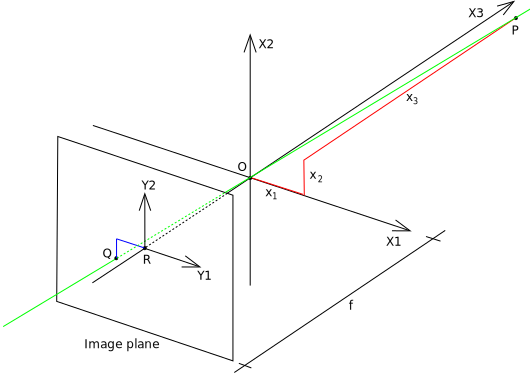
\includegraphics[width=0.8\textwidth]{pinhole3d}
}{fig:pinhole3d}{
	Pinhole camera geometry.
	Camera coordinate system origin and the physical pinhole at $O$, axis Z is parallel to the optical axis, U and V specify the image plane axes and the optical axis intersects the image plane at the principal point, the image center.
	The point $P = (P_x, P_y, P_z)$ projects to $p$, as well as everything else on the line joining them.
	The image plane is f units away from camera origin.
}

\paragraph{Projection}
Light rays travel through the pinhole camera's aperture to the image plane that is $f$ units behind the aperture, while the camera origin is set to the aperture \cite{hartley03multiview}.
This configuration is depicted in Figure \ref{fig:pinhole3d}.
The pinhole model (or, \emph{perspective projection}) states that the world point $(P_x, P_y, P_z)$ is projected via direct light rays to the 2D image plane at $(p_u, p_v)$:
\begin{equation}
\begin{pmatrix}
p_u \\ p_v
\end{pmatrix}
=
-\frac{f}{P_z} \begin{pmatrix}
P_x \\ P_y
\end{pmatrix}
\end{equation}
The result can be derived from similar triangles with a common vertex at the aperture.
Sometimes the sign is inverted, which results in a plane on the other side of the origin where the actual point lies, where the image is not rotated; this can be more convenient to analyse, since the image does not flip.
Physically, the projected point in a camera is behind the aperture, on the film or sensor.

% Matrices, homogeneous coordinates.
% projective element, "~" up to scale equality definition

\paragraph{Homogeneous coordinates}
In computer graphics and vision, points are usually described in \emph{homogeneous coordinates} \cite{dubrofsky2009homography,hartley03multiview,heyden2005multiple}.
An extra dimension is added to the interpretation of coordinates, and each point becomes a line that crosses the origin in a dimension one higher than the original.
Several vector operations become more convenient to manipulate: for example, 3D translation is embedded in 4D matrices with homogeneous coordinates.
The space is scale-invariant; all points $(xw, yw, zw, w)$ ($w \neq 0$) map to the same 3D point $(x, y, z)$.
This freedom of scaling makes many camera matrices defined only up to scale, as will follow.

%Homography definition (mapping of points and lines in $P^2$)

\paragraph{Camera parameters}
The imaging process essentially captures a projection to a flat two-dimensional plane of the camera's view.
When comparing points between different cameras that view the same scene, the cameras' relative positions and rotations must be known.
One of the cameras is often conveniently chosen as the origin of a global coordinate frame, so that its extrinsic parameters become unity transforms (many programming libraries may assume this, e.g., OpenCV \cite{opencv}).
%Each three-dimensional point in the world is transformed to the small sensor inside the camera, which is then digitized to a discrete two-dimensional grid of pixels, with different coordinate units.

The transformation chain \cite[p.~163]{hartley03multiview} is encoded as follows in Equation \ref{eq:projxform}, given a point $\vec P$ in homogeneous coordinates (4-dimensional vector) representing a 3D location described in physical (\emph{metric}) coordinates:
\begin{align} \label{eq:projxform} \begin{split}
	\vec p
	= \bm K_s \bm K_p \bm T \bm R \vec P
	= \bm K \bm T \bm R \vec P
	= \bm M \vec P
\end{split} \end{align}
where $\vec p$ is a 2D pixel in a discrete image, and $\vec P$ is still in physical units.
$\bm R$, $\bm T$ encode the camera rotation and translation (extrinsics) and transform the point to a camera-centric coordinate frame;
$\bm K_p$ projects the camera-centric world coordinates to the camera sensor (still in world coordinates), and finally the affine $\bm K_s$ transforms the points from the sensor to pixel coordinates on the digital image (not necessarily yet discretized).

The whole projection $\bm M = \bm K_s \bm K_p \bm T \bm R$ can be used as-is without decomposing it to separate matrices, unless the individual parameters are needed.
The matrices $\bm K_s$ and $\bm K_p$ are usually not decomposed but presented as a single intrinsic matrix $\bm K$, and $\bm R$ and $\bm T$ are usually given as a single extrinsic matrix.
As the chain consists of several matrices, some of them are defined only up to scale; the coordinate systems' units can be chosen freely.

The internal parameters, intrinsics, encode how the image is formed on the sensor: they consist of focal length $f$, pixel size ($m_x$ by $m_y$) and principal point $(u_0, v_0)$:
\begin{equation}
	\bm K =
	\begin{pmatrix}
		m_x & \gamma & u_0\\
		0   &    m_y & v_0\\
		0   &        0 & 1
	\end{pmatrix}
\cdot
	\begin{pmatrix}
		f & 0 & 0 & 0\\
		0 & f & 0 & 0\\
		0 & 0 & 1 & 0
	\end{pmatrix}
	=
	\begin{pmatrix}
		\alpha_x & \gamma   & u_0 & 0\\
		0        & \alpha_y & v_0 & 0\\
		0        & 0        & 1 & 0
	\end{pmatrix}
\end{equation}
For simplicity, the final matrix where pixel size and focal length are combined is often used.
Also, $\bm K$ is often given without the homogeneous part, as a $3 \times 3$ matrix.
$(u_0, v_0)$ specifies the image center (principal point).
The parameters can also be presented separately without the matrix notation.
For square pixels, $m_x = m_y$, and for a non-skewed (rectangular) sensor, $\gamma = 0$, which is often the case and assumed by computer vision programs and libraries \cite{hartley03multiview,szeliski10vision,heyden2005multiple}.

%Le image, Horizontal planar triangle, lines between camera origins etc, lecture11.pdf.

% }}} coord systems and transforms

\subsection{Camera calibration} % {{{

\emph{Calibrating} a camera means \emph{measuring} its intrinsic and extrinsic parameters in order to map its data to a known coordinate frame.
For only one camera, the camera itself could be chosen to be at the origin and its extrinsic parameters could be chosen as identity transform.
Intrinsic parameters are still necessary for knowning the projection.
For multiple cameras, one of them can be chosen as origin, the extrinsics of the others are then relative to that.
Calibration is not necessarily a manual step before scanning, but is still often performed with a physical calibration object if exact metric calibration is necessary.
Self-calibration and structure from motion techniques can recover camera calibration from a static scene automatically \cite{pollefeys1999hand,hartley03multiview}.

It is sometimes convenient to store intrinsics and extrinsics separately if the intrinsic matrix is constant for several pictures, for example.
The intrinsics need then be calibrated beforehand only once.
For a camera rig that does not change, whole intrinsic and extrinsic calibration can be retrieved beforehand and applied on further scanned datasets for direct reconstruction.

Manual calibration is done with a known pattern, such as a planar checkerboard pattern \cite{chuang2002performance,zhang2000flexible} or manually selected point pairs.
By knowing the geometry of the calibration object and the matching structure in the projected images, the projective transformation performed by the camera is obtained.
A known pattern is fast to detect and results in correct physical units when the physical pattern size is given.
% www.vision.caltech.edu/bouguetj/calib_doc/papers/zhan99.pdf

The checkerboard calibration step is often programmed to measure optical distortion at the same time \cite{opencv,camcalmatlab}.
A single image of a three-dimensional calibration object is also sufficient for single-camera calibration \cite[p.~181]{hartley03multiview}.

One general way for calculating the calibration is \emph{direct linear transform (DLT)}:
the whole matrix $\bm M$ is solved from $\vec x_i = \bm M \vec X_i$ by constructing a system of equations from the projections of some known points $i$, and minimizing an error metric, as the case is practically overconditioned and the measurements contain errors \cite{hartley03multiview}.
% XXX minimum number of points

A practical video-based method has been proposed by Svoboda for self-calibration \cite{svoboda2005convenient}.
The method uses a number of synchronized frames and a laser pointer in a dark calibration volume to automatically find corresponding points, not requiring any precise objects.

\emph{Structure from motion} (SfM) recovers full calibration for a larger amount of cameras with given matching point pairs, with no special requirements on the subject.
It can be used to calibrate an arbitrarily large unknown set of cameras automatically.
SfM is described further in Section \ref{sec:sfm}.

%many single planar chessboard pics vs a single image of an accurate 3d model.
%TODO Figure: show extrinsic in matlab cam calibs, nice pics (both cam and world centered)
%The scale of values affects the numerical calibration accuracy \cite{hartley1997defense,hartley03multiview}.
%A similarity transform is often initially applied to modify the values to a more consistent range.
%The 3D points are scaled accordingly, which is only ideal if the calibration object has uniform geometry \cite{hartley03multiview}.

% }}} camera calibration

\subsection{Calibrated stereo vision} % {{{

Given two or more views of a same scene, depth for a point can be extracted by comparing the positions of the point in different views.
Whole-picture depth extraction results in a depth map imaged from a single view, giving a depth value for each pixel in a picture, resulting in a set of three-dimensional points seen by that view.
In order to compare the point positions in two images, given a point in one image, its matching pair must be found on the other.
In the following section, this search problem in finding corresponding pixels, mapping them so that they can be compared, and the comparison that results a depth value is formalized.

% }}}

\subsubsection{Binocular disparity} \label{sec:binocular} % {{{

\simplegfx{t}{\textwidth}{simplestereo}{
	A stereo setup, pictured from above.
	The image planes (thick lines) are imaginary, as a real film in a camera would exist behind the camera origin and project the image as rotated around principal axis, as described earlier in Section \ref{sec:imaging}.
	The coordinates are given in units of the world coordinate system, common with the camera origins.
	The symbols $\vec C$ are the camera origins ($T$ units between each other), $\vec c$ the principal points, $x$ the one-axis image plane coordinates of $\vec p$ w.r.t.~the principal points, and $f$ is the focal length.
	The unknown is $Z$, i.e., depth of point $\vec X$.
}
% back planes to the figure? too much content then i guess

Assuming a planar setup with identical cameras (same focal length and sensor) with parallel optical axes as visualized in Figure \ref{fig:simplestereo}, a 3D point can be triangulated given its known projection on both cameras.
From similar triangles with a common vertex at $X$, the depth $Z$ is obtained as follows:
\begin{align} \label{eq:triangulation} \begin{split}
	\frac{Z}{T} &= \frac{Z-f}{T - x_l + x_r} = \frac{Z-f}{T - d}\\
	ZT - Zd &= ZT - fT\\
	Z &= \frac{fT}{d}
\end{split} \end{align}
The disparity $d$ is defined as the difference of the points in their image planes, $d = x_l - x_r$.
Note that $x_r < 0$ as it's to the left, towards to the negative axis, from the corresponding plane's origin.
It is not possible for $d$ to be negative.

%If the image planes would be fixed as being physically correct, in the back side of the camera origins, the focal length should be negated to keep the correct interpretation and sign because the projected physical image is mirrored in both axes.
%Image processing between the sensor and a picture file usually inverts this.
As Equation \ref{eq:triangulation} shows, depth is inversely proportional to pixel disparity in the images.
To map the depth to correct units, only focal length $f$ and the baseline $T$ are needed additionally; when using pixel coordinates instead of physical units in $d$, also the pixel size should be taken into account in scaling $x_l$ and $x_r$.
All of these are encoded in the camera parameters: the pixel size is part of the intrinsics, and the baseline is encoded in extrinsics.
Algorithms such as those in OpenCV \cite{opencv} can compute depth from disparity images based on the difference between each pixel.
The disparty image is a depth difference of each pixel value, which is calculated based on a correspondence search for each pixel;
more general camera calibrations and this search are discussed in the following.

% }}} binocular disparity

\subsubsection{Epipolar geometry} % {{{

\simplefig{t}{
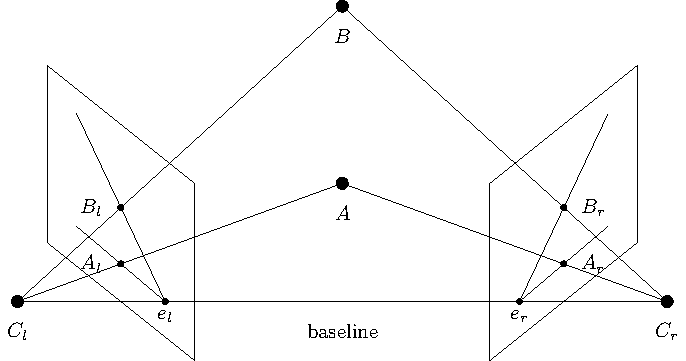
\includegraphics{epigeom}
}{fig:epigeom}
{Two camera views on same scene.
World points $A$, $B$ project to planes of different views imaged from $C_l$ and $C_r$ on the left ($A_l$ and $B_l$), and to the right ($A_r$, $B_r$).
The actual images cover some area of the total projection plane, and the epipolar point may or may not lie visible in the image.
When $A_l$ is known, its corresponding point $A_r$ (not initially known in practice) is found on the epipolar line joining $e_r$ and $A_r$ in the right image.
All epipolar lines in a view join in the same point ($e_l$ and $e_r$).}

% TODO: small algorithm for pairwise windowed point matching on the line (hox! and link to point matching section maybe)

In stereo vision, the same scene of interest is seen by two or more cameras at the same time.
The cameras are rarely aligned perfectly as in the stereo setup described above.
\emph{Epipolar geometry} \cite[ch.~7.3]{trucco1998introductory} encodes the relations between arbitrarily positioned cameras in a standard way so that coordinates of a 3D point seen in several images can be calculated with similar triangulation as in the simple stereo setup \cite{trucco1998introductory,hartley03multiview}.
As seen in Figure \ref{fig:epigeom}, a 3D point $\vec A$ seen by the left camera $\vec C_l$ could lie anywhere on the line between $\vec C_l$'s origin and $\vec A$, because a line passing through the principal point always projects to a point (the camera position is equal to the principal point, i.e., the pinhole).
This line is seen as a single point $\vec A_l$.
From another view, seen by the right camera $\vec C_r$, this line equals to some line on the right image plane.
The matching point must be on that line.
The inverse applies for any point on $\vec C_r$ and a line on $\vec C_l$.
These special lines on the image planes are called \emph{epipolar lines}, and they all coincide at a special point called \emph{epipole}, $\vec e_l$ and $\vec e_r$ (on the same plane as, but not necessarily inside, the projected image).
For example, the line from $\vec C_l$ to $\vec A$ projects to the line from $\vec e_r$ to $\vec A_r$ on the right plane, and likewise, the line from $\vec C_l$ to $\vec B$ projects to the line from $\vec e_r$ to $\vec B_r$, which can be easily seen from the triangles in the figure.

\emph{Essential matrix} \cite{hartley03multiview} describes how the camera poses differ, to match one image's point in another.
When $\vec A_l$, $\vec A_r$ specify the points in Figure \ref{fig:epigeom}, and the baseline difference is a vector from $\vec C_l$ to $\vec C_r$, it holds that
\begin{equation} \label{eq:esscrossprod}
	(\vec A_l-\vec C_l) \cdot (\vec C_r - \vec C_l) \times (\vec A_r-\vec C_r) = 0
\end{equation}
as all the vectors are coplanar.
The cross product yields a normal to the plane, which is perpendicular to all the vectors, and then the dot product equals zero.
In practice, the coordinates are given within the camera coordinate frames:
\begin{align*}
	\vec X_l &= \vec A_l - \vec C_l\\
	\vec X_r &= \vec A_r - \vec C_r\\
	\vec T &= \vec C_r - \vec C_l
\end{align*}
Then, Equation \ref{eq:esscrossprod} becomes
\begin{equation}
	\vec X_l \cdot \vec T \times \vec X_r = 0.
\end{equation}
Essential matrix $\bm E$ is a matrix form of this relation, and it provides a standard foundation on the epipolar geometry.
It includes the relative rotation and translation of the two cameras in a single matrix:
\begin{equation} \label{eq:essential}
	\vec A_l^T \bm E \vec A_r = 0
\end{equation}

\emph{Fundamental matrix} \cite[ch.~11]{hartley03multiview} is a similar object to essential matrix, as it also relates the corresponding points in stereo images.
It has the same meaning as the essential matrix, but it works in the pixel coordinates of the cameras.
The described vectors ($\vec X_l$, $\vec X_r$) are in normalized camera coordinate frames, but from the photographed images in actual image processing, only pixel values can be measured.
Thus, fundamental matrix encodes also intrinsic parameters.
Given pixel coordinates $\vec a_l$ and $\vec a_r$ that represent the points $\vec A_l$ and $\vec A_r$ as seen from cameras $\vec C_l$ and $\vec C_r$, respectively, the fundamental matrix $\bm F$ is given as:
\begin{equation} \label{eq:fundamental}
	\vec a_l^T \bm F \vec a_r = 0
\end{equation}

The essential and fundamental matrices can be seen as a more general configuration of the triangulation in Figure \ref{fig:simplestereo} and Equation \ref{eq:triangulation}.
The matrices can be estimated by forming a system of linear equations using Equation \ref{eq:essential} or \ref{eq:fundamental} and at least eight point correspondences, using some method to solve the equations, e.g., the \emph{eight-point algorithm} \cite[p.~155]{hartley03multiview}.
Having estimated the matrix, the epipolar geometry and thus the 3D position of any point with two matching pixel coordinates are easily recovered \cite[p.~162]{hartley03multiview}.

% }}} epipolar geometry

\subsubsection{Features and matching} % {{{

Previously, fundamentals for reconstructing a three-dimensional location for a point pair were introduced, assuming known positions for the same point in different images.
To reconstruct a whole scene from a full image, all pairwise points must be \emph{matched} \cite[ch.~4]{szeliski10vision}.
Matching is often also called \emph{correspondence} searching:
Given a pixel in one image, which is the corresponding pixel in another image taken from the same scene?
Pixels correspond to each other if they represent the same physical point.
Matching pixels for the previously introduced methods are found in the image space by comparing pixel intensity of some fixed window.
To describe the point's visual characteristics and to efficiently compare the characteristics of different points, the surrounding environment is typically encoded as a \emph{feature}, an easily recognizable property vector \cite[ch.~4]{szeliski10vision}.

For successful matching, and correct geometry, images from different views should represent the same object.
Different views must be imaged at the same time, and be free of visible view-dependent artifacts, such as specular highlights.
Artifacts may introduce outliers if matches are detected wrongly, or holes in the geometry if no matches are detected at all.

\paragraph{Features}
Edges or corners are the typical features that are detected automatically at specific steps of reconstruction.
They are essentially high-frequency information in the image that can be interpreted as a 2D discrete function;
thus, \emph{edge detection} can be performed by a discrete high-pass or band-pass filter, zeroing all but those pixels where a high difference is found \cite{marr1980theory}.
Another popular method is \emph{blob detection}, based on, e.g., the laplacian of a Gaussian-filtered image.
Blob detection is typically performed in computer vision using difference-of-Gaussian-based (DoG) methods due to its faster execution than in Laplacian-of-Gaussians \cite[p.~152]{szeliski10vision}.
Edge and blob detection methods work as a basis for several feature matching and detection algorithms.

\emph{Scale-invariant feature transform (SIFT)} \cite{lowe1999object} is a well-known algorithm for local feature detection and description.
A fast GPU implementation is also available \cite{changchang2007siftgpu}.
After detecting keypoint candidates with blob detection, SIFT encodes the local pixel neighborhood as a spatial histogram of gradients in the 2D image domain.
Invariance to scaling and rotation in feature descriptors such as SIFT make them useful in describing features that can be matched between unaligned images.

\paragraph{Search}
Searching for well distinguished features in an image is called \emph{sparse} search.
A sparse set of feature matches is suitable for reconstructing initial calibration, as all the feature vectors can be compared against each other relatively quickly.
For finding a complete depth map of the whole image, a slower \emph{dense} search is performed, using the obtained calibration.
Dense matching runs through each pixel of the search space and tries to find a matching pixel from another image, e.g., with template matching \cite{duda1973pattern}.
The surrounding pixel values themselves inside a \emph{window} centered at the searched pixel are compared in the search area, which typically runs along the epipolar lines only.

%From the coordinate differences in image space between the two images, a disparity map is built.
%The disparities can then be directly transformed to depth values, yielding a point cloud.
%Other more sophisticated algorithms too find dense matches but may not use an intermediate disparity map.

% }}}

\subsubsection{Image rectification} % {{{

% rectification pics

In order to triangulate a 3D point from two photographs, the location of the point in both images must be known, as described above.
Given a single pixel in one image, its corresponding pair would naively be searched by looking at every pixel in another.
Rectification is a process that simplifies this search problem by restricting the search to a single dimension using the epipolar lines \cite[p.~157]{trucco1998introductory} \cite[ch.~7.1]{pollefeys2004visual}.

A common \emph{planar rectification} projects the images on a common plane and rotates them such that corresponding lines are axis-aligned (horizontal or vertical) in both images \cite{hartley03multiview}.
By virtually aligning the cameras such that their images are coplanar and their axes parallel, the search only has to be performed on a line that is parallel to the line connecting the camera centers.
In Figure \ref{fig:rectification}, two cameras are situated at arbitrary positions, viewing different directions, and their view images are projected on a common plane, where they no longer are rectangular.
In practice, a new computer image is created that contains the projected image, and the search can be done along a single axis, or the search can be performed in the original image in the direction of the epipolar line.
Other more complex methods, e.g., polar rectification, can handle more general camera configurations \cite{pollefeys2004visual}.

\simplegfx{t}{0.5\textwidth}{rectification}{
	In planar image rectification, two images ($I_k$ and $I_l$) are projected to a common plane $\Pi_R$ as $I_k^l$ and $I_l^k$ respectively.
	The common plane is parallel to the baseline vector $\vec P_k-\vec P_l$.
	Image by Pollefeys \cite[p. 66]{pollefeys2004visual}.
}

% }}} correspondence and rectification

\subsubsection{Multi-view stereo} % {{{
% (trifocal tensor etc.?)

\emph{Multi-view stereo} (MVS) is stereo vision using more than two cameras.
In the research literature, MVS varyingly refers to both the big picture of a whole reconstruction pipeline using several pictures, and also just the dense reconstruction after system calibration has been done.
Reconstruction using a large set of cameras has two major choices:
One way is to extend the two-view geometry theory further to many cameras, recovering the whole subject at once using many views simultaneously.
Other very common method is to arrange the cameras in binocular pairs, reconstruct each pair separately to obtain a depth map from each pairwise view, and finally merge the resulting points to a single set.
Many of the following studies build a point cloud first and apply Poisson surface reconstruction \cite{kazhdan2006poisson} to recover a surface.

Okutomi and Kanade \cite{okutomi1993multiple} noted that a short baseline suffers from low precision and a longer one requires a larger space in searching and matching.
They approach the issue by combining several stereo pairs with different baselines, making correct point selection simple by using a minimized sum of errors.
A clear disadvantage of this approach is the increased number of cameras required.

The method by Fitzgibbon et~al.~\cite{fitzgibbon1998automatic} assumes a restricted geometry using a turntable with only single-axis rotational motion.
A single camera only is required, but the method does not extend to general cases.
The setting is comparable to a number of cameras photographing the subject arranged around it; surrounding geometry must first be removed.

Bickel et~al.~\cite{bickel2007multi} acquire a 3D face mesh surface with a commercial solution by 3dMD \cite{3dmd} and then apply basic triangulation methods on markers to track a deforming face and its wrinkles.
Their method uses a hybrid of fast low-resolution cameras for tracking and slower high-resolution cameras for recovering fine details.
Additional computation is done on post-processing the generated mesh.

Beeler et~al.~\cite{beeler2010high} perform a dense reconstruction in pairs using image pyramids and cross-correlation in block matching.
Normals on the points are computed using finite differences on disparity maps, and a surface mesh is computed using Poisson reconstruction.
The mesh is augmented with pore-level details assumed from lighting properties on surface microgeometry smaller than possible for normal disparity computation.

Bradley et~al.~\cite{bradley2010high} use seven stereo camera pair arrangements directed to different parts of the subject, and combine the resulting 3D point clouds into a single one for meshing and animating with optical flow.
The geometry is tracked by using optical flow to compute vertex positions between successive frames.
An initial mesh is computed and manually refined, which is then modified preserving the vertex connectivity.
Too fast movement not suitable for optical flow is tracked separately with a priori knowledge of the subject, such as special constraints on a human mouth.

Ghosh et~al.~\cite{ghosh2011multiview} compute a single output directly with no merging of intermediate point clouds by assuming that the subject is a deformed cylinder.
The cylinder is subdivided in small parts that individually deform based on the captured data, which easily preserves the subject structure.

The large-scale approach by Snavely et~al.~\cite{snavely2006photo} presents methods and user interfaces that are not restricted on pre-calibrated or pairwise cameras, but instead are designed for unordered image collections.
The method presents only the structure from motion solution and is suitable for thousands of views.

Toldo et~al.~\cite{toldo2013accurate,toldo2013towards} present an algorithm with visibility constraint filtering on a point cloud combined from a disparity map on each camera, with no requirements on camera structure such as pairing.
The point cloud is converted to a mesh with Poisson surface reconstruction.

A global \emph{surface element} (\emph{surfel}, \emph{patch}) approach is used by several researchers recently \cite{carceroni2002multi,furukawa2010accurate,vu2012high,chang2011gpu}.
The surface is not interpreted as a simple point cloud, but as a surface consisting of small elements, each visible in several views.
Visibility constraints can then be employed based on occlusion between the elements and the outliers can be filtered away effectively.

The patch-based method by Furukawa et~al.~\cite{furukawa2012patch,furukawa2010accurate} collects initial correspondences from all source images, and expands 3D patches to a dense set iteratively spreading current matches to nearby pixels, finally filtering them by visibility constraints globally.

Energy minimization with graph cuts applied in computer vision \cite{boykov2004experimental} is also increasingly used in dense reconstruction \cite{chang2011gpu,vu2012high,labatut2009robust,jancosek2011multi} for labeling the depths in a discrete voxel grid or a triangulation.

% }}} multi-view stereo

\subsection{Structure from motion} \label{sec:sfm} % {{{


The \emph{structure from motion (SfM)} problem, also called \emph{structure and motion}, uses the scene feature matches between different views to determine both the scene structure and the camera motion between the views \cite{snavely2006photo,fitzgibbon1998automatic,pollefeys2004visual}.
The camera does not have to physically move; the method can be used for multi-camera reconstruction with a static rig.
Before SfM, the images must be undistorted and features matched; the algorithm works on point locations instead of input images.
While SfM retrieves the scene structure and camera parameters, a dense reconstruction usually follows it as only a fraction of the points in the images need to be considered \cite{pollefeys2004visual}.

SfM begins with two reference views that are used to retrieve an initial reconstruction, and extends each new view into the set iteratively.
A \emph{bundle adjustment} method is used to globally optimize the scene parameters \cite{triggs2000bundle}.
Many reconstruction programs use structure from motion as an initial step to determine calibration and proceed then to dense reconstruction.

The initial stage builds a reference frame and structure for the selected features (points) in two cameras.
The structure is determined with triangulation as in Section \ref{sec:binocular}.
In practice, perfect reconstruction cannot be achieved due to noise, and the points are found by minimizing a reprojection error to the extent of a specified threshold limit.

After a coordinate frame is built as a basis using two views, the next camera views are iteratively added to obtain an initial estimate of the camera poses and the selected scene feature positions.
Scene features can be matched between only last few views if the camera motion is known to be continuous;
the matches can also be done between all possible image pairs, which is useful if there is overlap.

As a last step, bundle adjustment globally optimizes the \emph{bundles of light rays} from the scene to all cameras.
Several algorithms and implementations are available, while the basic idea and the underlying problem is the same:
a cost function is used to optimize jointly all camera parameter estimates such that the reprojection errors are minimized through all views.
Pollefeys \cite{pollefeys2004visual} gives the following formula to minimize:
\begin{equation}
	\text{min}_{\bm M_k, \vec P_i} \sum_{k=1}^m \sum_{i=1}^n D(\vec p_{ki}, \bm M_k \vec P_i)^2
\end{equation}
when the goal is to find the projection matrices $\bm M_k$ and the 3D points $\vec P_i$ for all views $k$ and points $i$, where $D(\vec a,\vec b)$ is the Euclidean distance between $\vec a$ and $\vec b$ and $\vec p_{ki}$ the known, fixed matching 2D image position in the $k$th image for the unknown 3D point $\vec P_i$.
In practice, this nonlinear optimization problem is approached in iterative means.
According to Wu \cite{wu2013towards}, bundle adjustment should be performed using a Levenberg-Marquardt or Preconditioned Conjugate Gradient method.
%Beardsley et~al.\ use an iterative extended kalman filter \cite{beardsley1997sequential}

An incremental algorithm linear-time in number of the cameras has been suggested for structure from motion for large-scale reconstructions \cite{wu2013towards}.
A specialized scanning rig in this work is not considered large-scale.
Large-scale refers to hundreds or even thousands of images of a huge geometry, such as an outdoor building or terrain.

% }}}

\subsection{Error metrics} % {{{

The quality of the reconstruction is measured by reprojecting the 3D points back to the cameras with the estimated parameters, and calculating the distance between the projected and the matching original point, the \emph{reprojection error}. \cite[p. 95]{hartley03multiview}

Furthermore, if the scene structure is known beforehand (e.g., as a calibration object, whose physical properties are measured), the resulting quality of the structure can be compared to ground truth.
Ground truth data can also be obtained with a real 3D scanner, such as a laser ranging device. % david

In addition, uncertainty in depth depends more heavily on the pixel errors (i.e., disparity precision) if the baseline is short, as depicted in Figure \ref{fig:baselineerr}.
The ability to discern the position of tiny features in images is some absolute value in pixel units.
When the disparity approaches the scale of this uncertainty, it becomes increasingly difficult to extract an accurate value for depth.
Given an absolute uncertainty $\Delta d$ for the measured disparity $d$, the error
\begin{equation}
	\frac{\partial}{\partial d} Z \Delta d =
	\frac{\partial}{\partial d} \frac{fT}{d} \Delta d =
	-\frac{fT}{d^2} \Delta d
\end{equation}
clearly increases quickly as the measured disparity $d$ becomes smaller.

\simplegfx{t}{\textwidth}{baselineerr}{
	The effect of baseline difference $||\vec A - \vec B||$ on the depth error $Z_2 - Z_1$, with a small (left) and large (right) baseline.
	Point $\vec P$ is seen by the two cameras $A$ and $B$.
	Points $\vec P_l$ and $\vec P_r$ depict the left and right possible points on the raster image, i.e., the possible range for the pixel.
}

When sparse feature matches are searched for matching picture points in different views, a number of features are first generated for each picture, and the matches are tested against picture pairs.
False positive matches should be filtered out; common way to handle feature outliers is Random Sample Consensus (RANSAC).
Random subsets of the sample space are iterated, and samples that do not fit well to a model (i.e., the camera parameters) that is constructed for a smaller set are ignored.
The iteration that matches most samples is selected. \cite{hartley03multiview}

%Detail calculation (error on surface ~= avg reprojection error?) compute millimetres

Practically, the scale of the camera sensor size and focal length in physical units (millimetres) are often known, making conversion from pixel units to millimetres possible.
Units originating from reconstruction of raster images can be simply scaled to millimetre units, resulting in more intuitive error interpretation.

%Compare to algebraic, geometric etc.

% }}}

\subsection{Surface fitting} % {{{

A multi-view reconstruction results in a discontinuous set of three-dimensional points, with no \emph{connectivity information}, i.e., interpretation of \emph{surfaces}.
In reality, all the pixels are projections of nearby surfaces, and a more natural and standard representation is obtained by fitting a surface on the points.

Computer graphics typically uses data structures based on piecewise surfaces \cite{foley1990computer}.
The surfaces are described as collections of small patches with a polygon outline.
When ultimately rendering the polygons on a computer screen using the graphics processing unit (GPU), pixels inside them are interpolated to contain all color information available in the source photographs.
%Coloring the surfaces is known as \emph{shading}, and modern GPUs run \emph{shader programs} given by a programmer or an artist and specially crafted for a purpose, such as rendering photorealistically using detailed lighting models.
%Lighting models typically use several spatially varying parameters that describe parameters such as the surface color, roughness and glossiness.

% }}} surface fitting

\subsubsection{Data structures} % {{{

\simplefig{t}{%
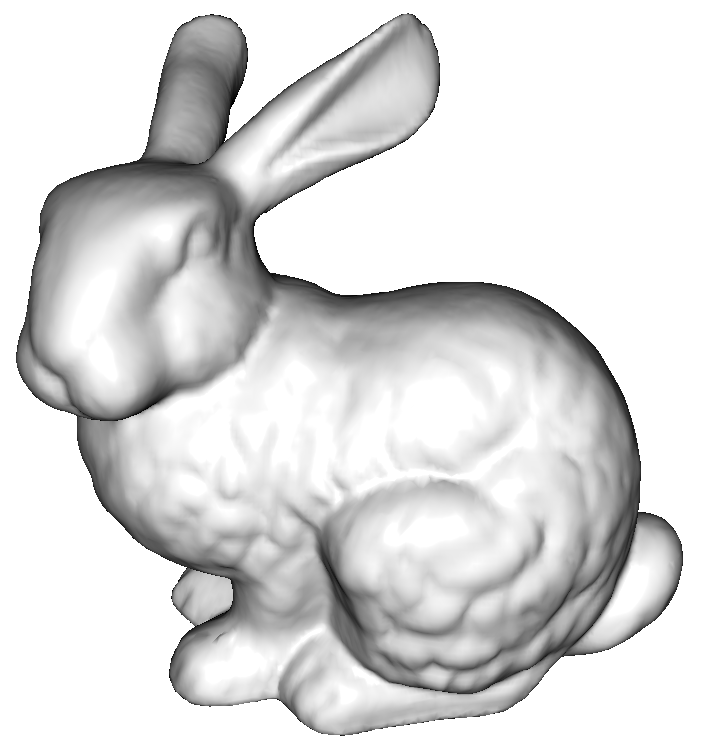
\includegraphics[width=0.3\textwidth]{bunny}
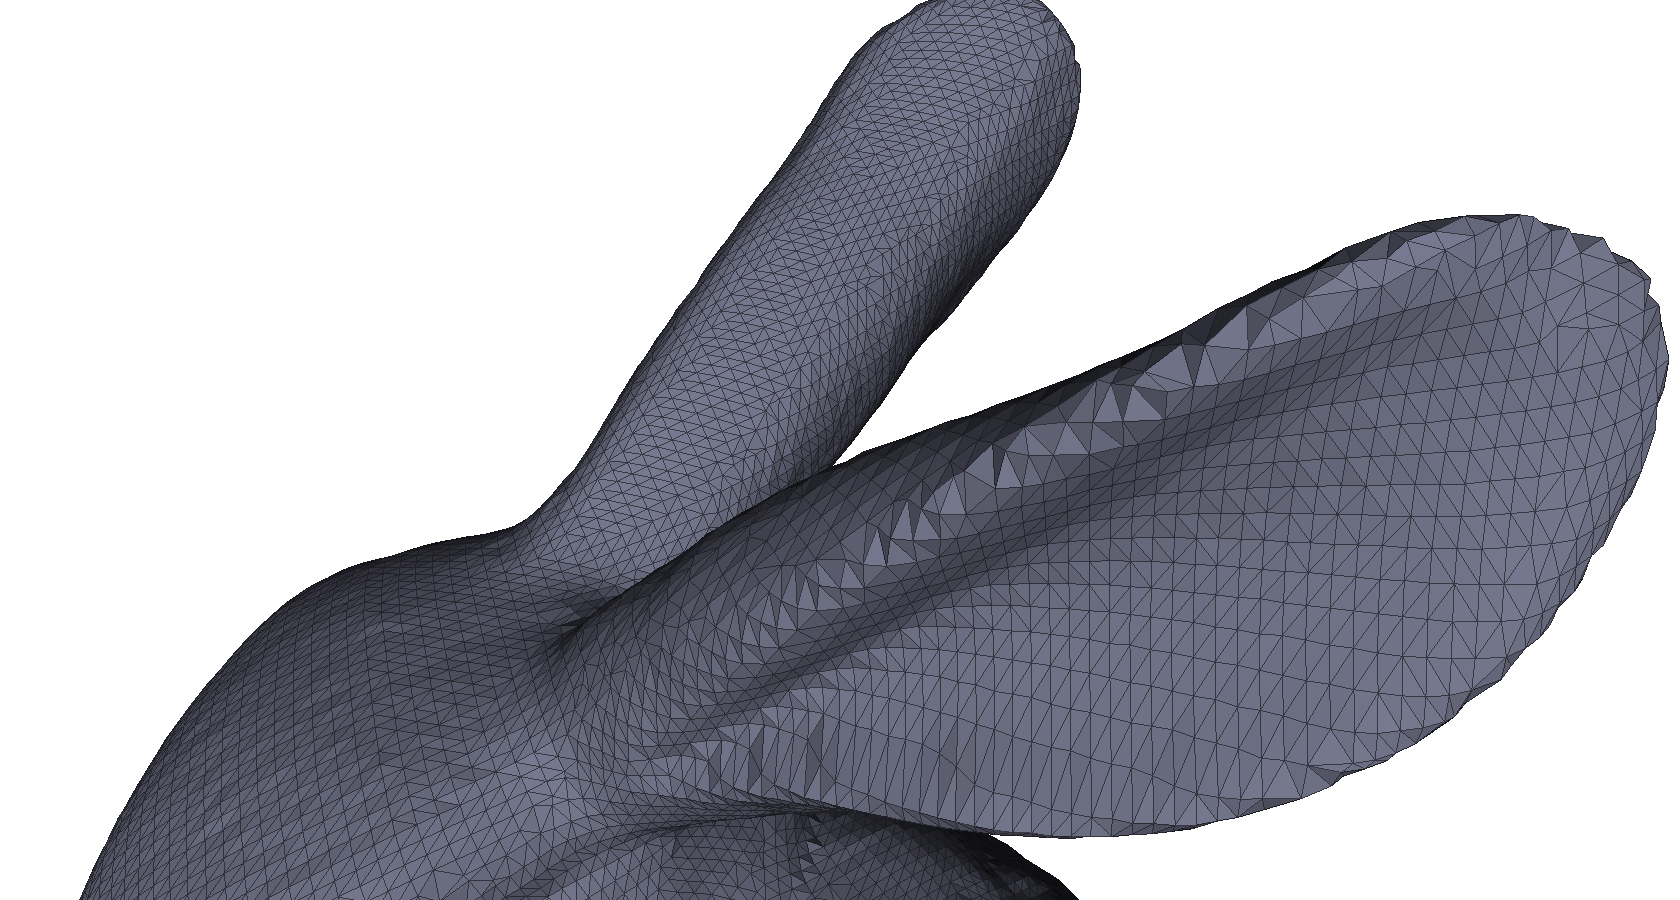
\includegraphics[width=0.6\textwidth]{bunnyear}
}{fig:stanfordbunny}{
	Stanford Bunny, a standard 3D test model by The Stanford 3D Scanning Repository, Stanford Computer Graphics Laboratory, scanned with a laser ranger.
	On the left: the whole model, shaded with a simple Phong lighting model.
	On the right: a closeup of the left ear, showing the edges of the faces as black lines connecting the vertices.
}

A \emph{(polygon) mesh}, a data structure often used to describe 3D models, consists generally of \emph{vertices} connected by \emph{edges}, forming \emph{faces} of objects \cite{foley1990computer}.
The meshes often consist of triangles, which is the simplest possible polygon.
Polygon meshes have a \emph{topology}; the connectivity information of vertices on a surface, describing neighbours of each point.
Surface \emph{normals} describe the orientation of the polygon patches.
Normals are important in rendering the surfaces realistically in any given lighting environment.
Figure \ref{fig:stanfordbunny} depicts the vertex structure of a typical 3D model.

A \emph{point cloud} is a loose term for a disorganized set of 3D points with no topology information, i.e., a cloud consists only of a list of vertices, with possibly some attributes such as colors or normals.
Point cloud is a natural output format for 3D reconstruction, as each point in the cloud maps to some pixel in a source image.

% }}} data structures

\subsubsection{Geometry} % {{{

Assuming that the recovered 3D point cloud represents the surface of an object, the next step of interest is to recover the surface topology from the point cloud.
The point cloud is all geometric information that is available, but the images probably consist of more pixels than the number of points in the point cloud.
To work with the generated model and to render it properly with colors, it is desirable to recover the topology information.

A popular method for surface reconstruction from a point set is \emph{marching cubes} \cite{lorensen1987marching}.
The algorithm builds triangles in a divide-and-conquer approach based on whether points are inside or outside a cube in a hierarchial grid.
A number of surface recovery methods have been proposed that utilize marching cubes as a final step.
The algorithm of choice is currently \emph{Poisson surface reconstruction} \cite{kazhdan2006poisson,kazhdan2013screened}.

Before fitting a surface on the points, the point data set should be processed either manually or automatically to remove outliers, such as wrongly detected points or geometry of the surrounding scene not part of the object itself.
Specular highlights and other artifacts on the surface may also introduce outliers.
Manual work in a point cloud editing software is a simple way to delete the points that are not part of the actual object.
If manually filtering the subject would be undesirable, e.g., when recording many expressions on a human face in a constant environment or rendering the scan in realtime, automatic methods could be used, e.g., nearest-neighbor or point grouping methods \cite{pcl}.

% }}} geometry

\subsubsection{Texture reprojection} % {{{

When a polygon mesh is available, it should be rendered in color, including the areas between the original points.
The de facto method in computer graphics is to uses \emph{texture mapping} to color pixels in between the vertices, when the number of vertices is less than the number of pixels on the screen.
A \emph{texture coordinate} is set for each vertex in the mesh to \emph{map} a smaller image from the texture on to the particular polygon. \cite{foley1990computer,heckbert1986survey}

Building the texture is done in a similar way of rendering the image on a screen or capturing a scene with a camera:
The reconstructed mesh surface is projected on the raster images, registering the image coordinates on each vertex \cite[p.~610]{szeliski10vision} \cite[p.~98]{heyden2005multiple}.
When the mesh is viewed from another viewpoint, the pre-projected texture data is used again.
Great accuracy can be acheived if a MVS structure is combined with a laser scan, by registering the point clouds generated by both together, using the laser scan as geometry and registered camera poses to project textures \cite{liu2006multiview}.
% (XXX meshlab src, references?)
% note: parameterization + texturing from registered rasters

When several cameras share the same view, the correct texture must be chosen on each vertex.
The selection can be taken based on some goodness criteria, e.g., the image with largest viewed area or highest brightness.

\simplegfx{t}{\textwidth}{texreproj}{
	Texture mapping a triangle from a color image on a virtual image plane on a computer screen as $m_v$.
	The triangle geometry is mapped on the color images, or textures, of the real cameras as $m_i$, and the triangular patch between the image vertices is stretched on the rendered triangle.
	Image from \cite[p.~98]{heyden2005multiple}.
}

To optimize the triangle rendering resources of GPUs, the deepest level of geometry is typically colored using texture maps describing not color, but \emph{surface roughness} and \emph{glossiness}.
Accurate lighting models make heavy use of highly spatially varying surface \emph{normals} and microgeometric details, instead of the absolute position of the geometry.
Such information is typically kept in a \emph{normal map} or a \emph{bump map}, encoding the surface normal or roughness at each visible pixel.
Several studies have presented methods to augment the base geometry by adding wrinkles as normal mapping \cite{bickel2007multi}.

\clearpage
\section{Motion capture} \label{sec:motioncapture} % {{{

\emph{Motion capture} (mocap, or mo-cap) is the practice of recording object movement over time.
A recorded subject can be described as a piecewise rigid object, e.g., a human, possibly encoding also some skin movement.
In computer animation, the movement data is encoded as positions of certain vertices at each recorded point in time, and often post-processed to be parameterized by joint angles or muscular actions \cite{deng2007computer,waters1987muscle}.
\emph{Surface capture} is a related term referring to a similar motion recording but happening on a deforming surface instead of globally moving rigid bodies.

% }}} mocap

\subsection{4D data capture} % {{{

The term \emph{4D} in the reconstruction context refers to temporally varying 3D data.
Analogous to the case of traditional 2D video consisting of separate discrete frames of pixels, a sequence of dynamic 3D data is, in a simple case, individual ``frames'' of point clouds.

For source data in the form of video files per camera, effectively a sequence of sets of synchronized pictures, each set of frames can be considered a static geometry on which the reconstruction would be done.
A naive alignment to previous or first frame is possible to average out the object movement if only its local surface movement is of interest.
Still, reconstructing each point in time separately would not necessarily produce the same topology for the mesh.
Each frame would produce a different point cloud not connected to the previous reconstruction, unless some algorithm that takes this into account is used.

Possibilities to correct the lack of coherent geometric structure exist.
Typical methods include fitting each frame of the mesh to another pre-recorded or pre-modeled mesh \cite{bickel2007multi,bradley2010high,li2009robust,zhang2007spacetime} and matching to the previous frame iteratively, or using intermediate keyframes for later animation \cite{beeler2011high}.

% }}}

\subsection{Geometry tracking} % {{{

%Kalman
%Fiducials / AR
%perf of cloth anim capture
The applications of dynamic reconstruction require tracking of individual points or objects in order to usefully handle the moved subject, as the applications typically require a known model whose movements are recorded.
A new model for each frame would not be suitable.
Non-static human motion capture in video gaming or movies, where post-processing time is available, can rely on manual work to perfect the quality.
In realtime applications, the full frame is typically not reconstructed again, but only selected keypoints that are tracked in 2D are triangulated, and a previously scanned model is deformed based on them.

However, the simplest tracking method is to leave tracking out completely: depending on the application, tracking might not be needed if the work done on the three-dimensional data does not need topological coherence in the time domain, but recomputes its work on each new point cloud.

In three dimensions, a template model is often scanned beforehand that is then morphed to match the target object to keep the topology (i.e., vertex neighborhood connectivity) constant.
This technique adapts well to non-rigid deforming subjects \cite{bojsen2012tracking,li2009robust}.
Starck et~al.\ \cite{starck2007surface} use a different approach with the same topology-preserving idea by subdividing a sphere and mapping it on the scanned subject.
A similar method is used by Ghosh et~al.\ \cite{ghosh2011multiview} using a cylinder instead of a sphere.
Common application also for the entertainment industry is \emph{animation retargeting}: using a completely separate character, and deforming it on each frame based on the current state of the scanned object, fitting the model's vertices to the scanned set \cite{sumner2004deformation}.
% siggraph14 doghead

Sometimes the computer animation must be optimized for feasible playback, such as reducing the amount of data required, or making it easier for humans to adjust the animation by parameterized models.
Parameterized models may include a base template pose and spatially varying deformations such as muscle models warping groups of vertices \cite{waters1987muscle}, or completely separate keyframes such that the animation is interpolated as linear combinations of different poses \cite{deng2007computer,beeler2011high}.

% }}} geometry tracking

\subsection{2D surface tracking} % {{{

%* SIFT/SURF/Harris feature tracking, reproject
%* edgels (edge pixels)

In two dimensions, the dense reconstruction step can be skipped when using only features in image space, providing real-time performance \cite{pilet2005real}.
Assuming that a particular object stays in the imaged volume, features can be detected and mapped to a point on the 3D surface, and tracked locally with no full-image reconstruction, while the tracked object is assumed to keep the same topology as a previously scanned template model.

Classic motion capture uses special reflective markers that are tracked in 2D with infrared cameras.
Distinctive bright markers are easily thresholded from the background, tracked, and triangulated in real time.
Markerless surface capture detects image features that are then used as virtual markers, working in a similar way.
Matching textured objects is more computationally intensive, and needs high resolution cameras \cite{moeslund2001survey}.
Markerless capture is important in scanning facial movement, because time-varying texture is significant in highly dynamic and detailed deformations, such as wrinkles from different facial expressions \cite{bradley2008markerless,beeler2011high,bradley2010high}.

Tracking is done by looking for the same feature as in a previous frame in the neighborhood where it was previously.
State-of-the-art 2D tracking methods include Kanade-Lucas-Tomasi (KLT) \cite{lucas1981iterative,tomasi1991detection}, Tracking-Learning-Detection (TLD) \cite{kalal2012tracking}, and Consensus-based Matching and Tracking (CMT) \cite{nebehay2014consensus}, all based on \emph{optical flow} \cite{horn1981determining,gibson1950perception,beauchemin1995computation}.
Given source and destination images, optical flow is the apparent motion in the scene between the images, given as a motion vector for each pixel.
Estimating the flow is based on the brightness constancy constraint: the intensity of the source and destination pixels is the same \cite{horn1974determining}.

Optical flow is also used in interpolating new frames between recorded frames for non-synchronized cameras \cite{bradley2009synchronization,eugster2011slowmovideo}.
The assumption of stereo reconstruction that the cameras encode the same scene can then be virtually achieved by interpolating the motion vectors between two frames to obtain an intermediate frame that then temporally matches that of another camera.

% }}} 2d tracking

\subsection{3D registration} % {{{

Aligning two meshes or point clouds together is called \emph{registration} in three dimensions \cite{zhang1994iterative,rusinkiewicz2001efficient}.
Registration finds a rigid transformation from one object to another.
For a moving subject, the method can be used to find the object movement between the frames \cite{pons2005modelling,zhao2005alignment}.
Registration is also used for combining different, overlapping parts of a static subject generated from different viewpoints to one larger model if the number of cameras is not enough for complete surface coverage \cite{eggert1998simultaneous,huber2003fully}.

The basic idea in registration is to fit two surfaces or point clouds together so that the shapes that they present become as close as possible to each other.
The practical method of choice is iterative closest point fitting (ICP).
Given a sufficiently close initial guess, ICP iteratively finds a rigid transformation that minimizes the distance between every point in one mesh and its closest match in the other.
In tracking applications, an identity transform is a good initial guess for the algorithm, because the tracked object has presumably moved only a little.
Variants of the original ICP apply assumptions on real-world data and errors, to improve convergence speed and quality \cite{zhang1994iterative,rusinkiewicz2001efficient}.
Advances to the rigid ICP has been proposed to address surface noise and other issues, by applying ICP locally and allowing the surfaces to warp \cite{brown2007global}.

% }}} registration
